\chapter{Literature Review}
\label{ch:LiteratureReview}

\section{Image Evaluation}
\label{sec:ImageEvaluation}
There are three ways to evaluate an image: assessing its quality, aesthetics, or fidelity. Each method focuses on different aspects of image evaluation and has unique applications. \par
\vspace{\baselineskip}
\noindent
\textbf{Image Quality Assessment} (IQA) measures the degradation of an image. This involves comparing an original, undistorted image with a processed version that has undergone changes such as compression, noise addition, or artifact introduction. The goal is to quantify how much the image quality has declined due to these changes.\par
\vspace{\baselineskip}
\noindent
\textbf{Image Aesthetics Assessment} focuses on the visual appeal of an image. It evaluates how pleasing an image is to the human eye, considering factors like composition, color, and overall aesthetic impact. While related to IQA, since both involve human judgment, this area is not the focus of this thesis because it deals more with subjective perceptions of beauty rather than measurable quality degradations. \par
\vspace{\baselineskip}
\noindent
\textbf{Image Fidelity Assessment} deals with how accurately an image represents the original scene or view. This is especially relevant in applications involving multiple views or stereo cameras, assessing the correctness of image reconstruction. However, this thesis will also not cover image fidelity assessment, as it pertains more to the accuracy of recreating an image rather than evaluating its quality after processing. \par
\vspace{\baselineskip}
\noindent
The primary focus of this thesis is on IQA, specifically looking at various types of image degradation. The following subsections will discuss common distortions, datasets that contain these distortions, and the state-of-the-art (SOTA) methods in IQA. But first, it is important to distinguish between subjective and objective quality assessment. \par


\subsection{Subjective Quality Assessment}
\label{sub:SubjectiveQualityAssessment}
Subjective quality assessment involves human observers evaluating the quality of images based on their visual perception. This method is essential for understanding how humans perceive image quality in real-world situations, especially when technical measurements might not fully capture what people actually see and experience. There are two primary methods used in subjective quality assessment:\par
\begin{itemize}
    \item Absolute Categorical Rating:  In this approach, human observers are presented with a unlabeled image and asked to rate its quality based on predefined categories. Each observer evaluates the image independently, without comparing it to any reference image. This method allows evaluators to provide a direct judgment on the image’s quality based on their subjective experience.
    \item Paired Comparison:  In this method, human observers are presented with two images: a unlabeled image and a reference image. Observers then assess the quality of the test image by comparing it directly to the reference image, assigning a score based on the perceived differences in quality.
\end{itemize}
Subjective quality assessment is highly valued for its ability to accurately reflect human perception of image quality. However, this method is also resource-intensive, requiring significant time and effort from human evaluators. Additionally, subjective assessments can be influenced by variability and biases introduced by individual scorers. For example, differences in monitor color calibration, the scorer’s domain knowledge, and personal preferences can affect the consistency and reliability of the evaluations. Despite these challenges, subjective quality assessment remains a critical component of comprehensive image quality evaluation, particularly in applications where the human response to an image is the ultimate measure of its quality. \par

\subsection{Objective Quality Assessment}
\label{sub:ObjectiveQualityAssessment}
Objective quality assessment relies on mathematical algorithms rather than human judgment to evaluate image quality. This approach uses our understanding of human vision system attributes to develop mathematical equations that measure quality, even though not all methods rely on these attributes. Essentially, it involves comparing data points or features extracted from images to determine quality. This assessment is mainly categorized into three methods based on the reference data used: Full-Reference IQA (FR-IQA), Reduced-Reference IQA (RR-IQA), and No-Reference IQA (NR-IQA). \par
\vspace{\baselineskip}
\begin{figure}[ht]
    \centering
    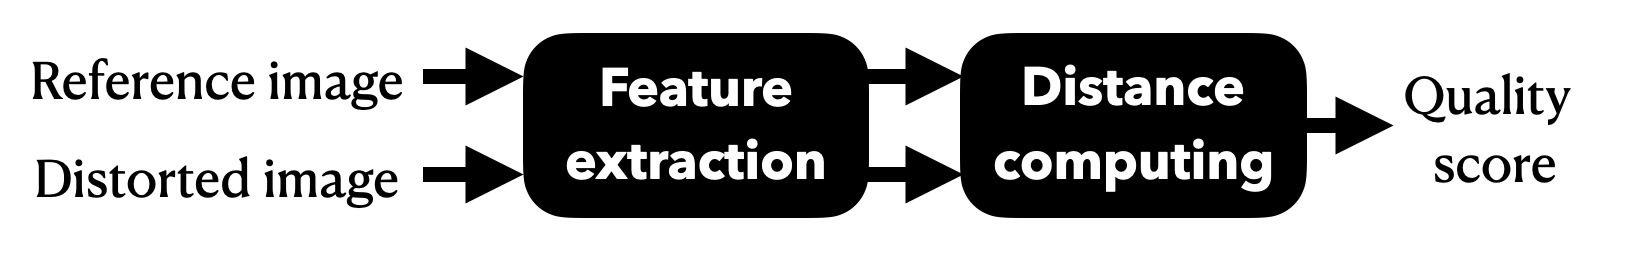
\includegraphics[keepaspectratio,width=15cm]{img/FRIQA.jpg}
    \caption{General framework of FR-IQA algorithms. Features are extracted from both images, and then the feature distance is calculated.}
    \label{fig:FRIQA}
\end{figure}
\noindent
\textbf{Full-Reference IQA} (FR-IQA) involves a comprehensive comparison between a distorted image and a reference image (see \autoref{fig:FRIQA}). Features are extracted from both images, and their differences are quantitatively analyzed to compute a quality score. While FR-IQA offers detailed assessments, it requires a reference image for every distorted image evaluated, which can limit its practicality. \par
\vspace{\baselineskip}
\begin{figure}[ht]
    \centering
    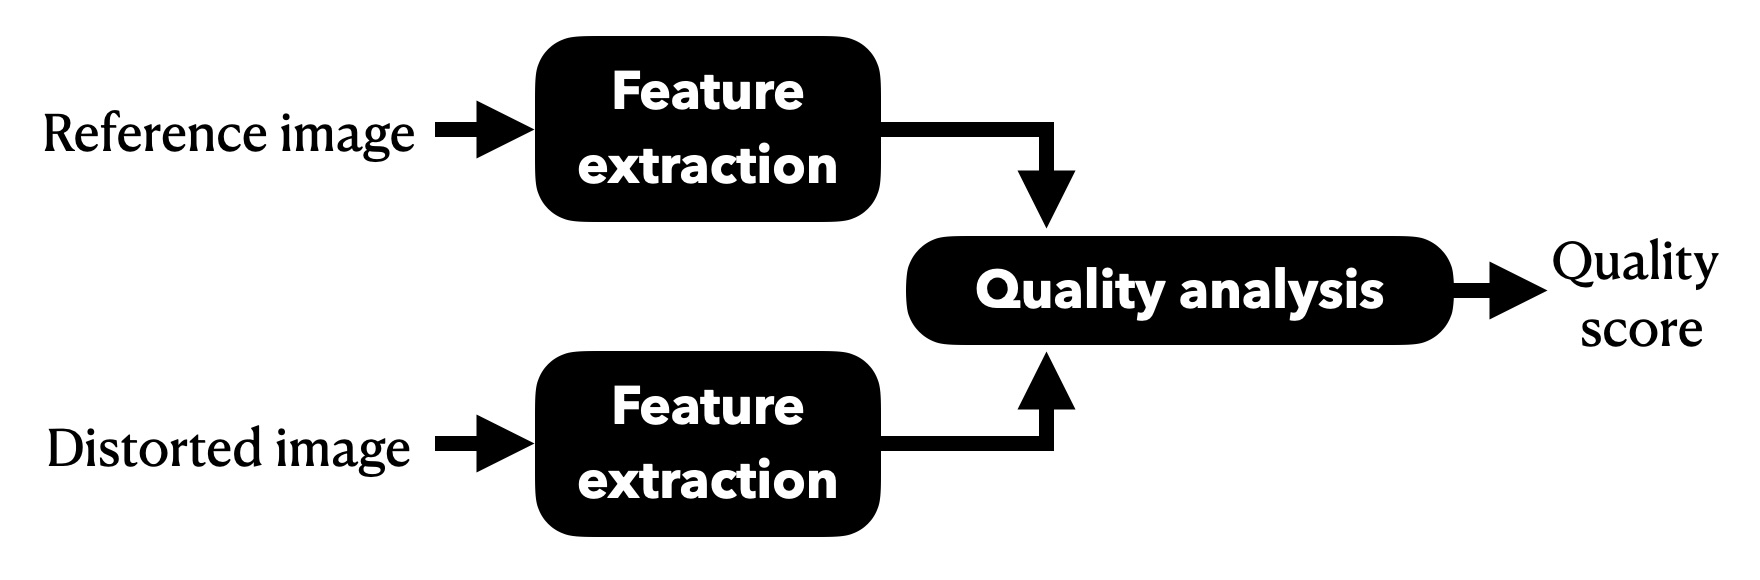
\includegraphics[keepaspectratio,width=15cm]{img/RRIQA.jpg}
    \caption{General framework of RR-IQA algorithms. Features of the reference and distorted images are extracted and used collectively to compute the quality.}
    \label{fig:RRIQA}
\end{figure}
\noindent
\textbf{Reduced-Reference IQA} (RR-IQA) operates similarly to FR-IQA but does not need the complete reference image. Instead, it uses a reduced set of features extracted from both the distorted and reference images (see \autoref{fig:RRIQA}). This method balances the exhaustive comparison of FR-IQA and the independence of NR-IQA, reducing computational demands while still providing meaningful quality assessments based on partial reference data. \par
\vspace{\baselineskip}
\noindent
Both FR-IQA and RR-IQA utilize two methods to analyze quality:
\begin{itemize}
    \item Spatial-Based Analysis: This method compares images pixel by pixel or region by region, offering straightforward interpretation and efficient computation. However, it may not fully align with how humans process images, lacking robustness in some scenarios.
    \item Transform-Based Analysis: This approach transforms images into a different domain (such as the frequency domain) that more closely mimics the human visual system. While robust, it is complex and computationally intensive.
\end{itemize}
\vspace{\baselineskip}
\begin{figure}[ht]
    \centering
    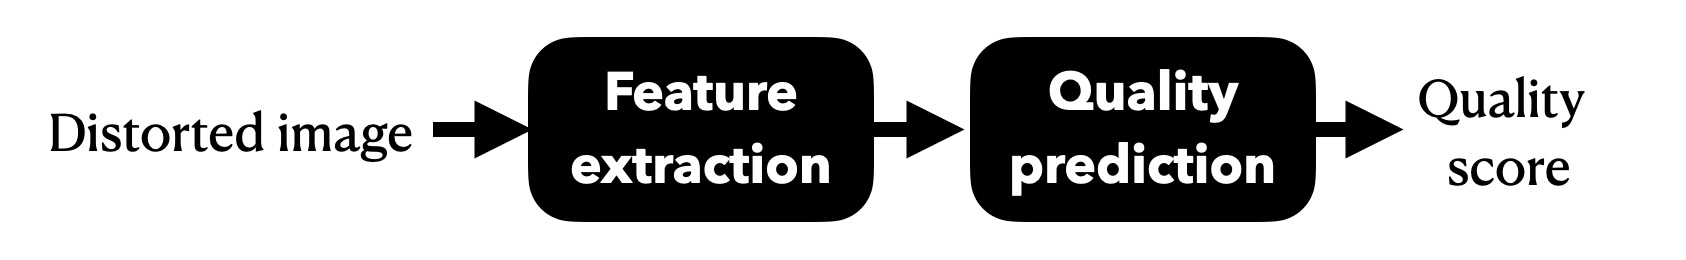
\includegraphics[keepaspectratio,width=15cm]{img/NRIQA.jpg}
    \caption{General framework of no-reference image quality assessment algorithms.}
    \label{fig:NRIQA}
\end{figure}
\noindent
\textbf{No-Reference IQA} (NR-IQA) does not rely on any reference image. Instead, it analyzes the distorted image alone by extracting features indicative of quality (see \autoref{fig:NRIQA}). This method is particularly useful when no reference images are available, such as in many practical applications of teledermatology. NR-IQA can be tailored to address specific types of distortions or designed for general-purpose quality assessment, providing versatility across various domains. \par
\vspace{\baselineskip}
\noindent
For this thesis, the focus will be on No-Reference IQA because it is especially relevant for evaluating teledermatology images where reference images are usually not available. Since IQA measures distortions and NR-IQA can handle various types, it is important to identify the most common distortions encountered. The next subsection will discuss these distortions in detail. \par

\subsection{Common Distortions in Image Quality Assessment}
\label{sub:CommonDistortionsIQA}
mage Quality Assessment (IQA) must address various distortions that can significantly affect the perceived quality of images. Understanding these common distortions is crucial for developing effective IQA algorithms, particularly in contexts like teledermatology, where accurate image assessment is critical. Below are the common distortions typically considered in IQA, with a reference image shown first for better comparison: \par
The common distortions are:
\begin{figure}[ht]
    \centering
    \begin{subfigure}[b]{0.24\textwidth}
        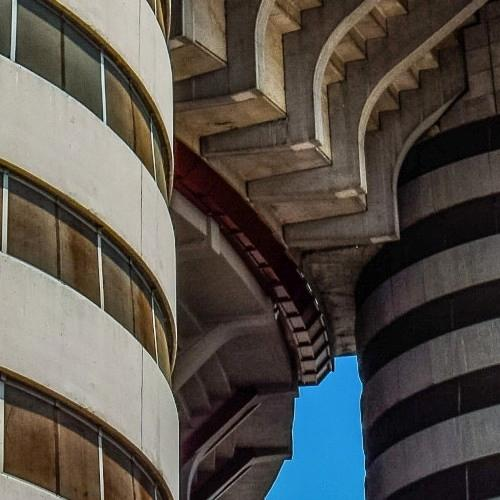
\includegraphics[width=\textwidth]{img/Original.jpg}
        \caption{Original}
    \end{subfigure}
    \hfill
    \begin{subfigure}[b]{0.24\textwidth}
        
\includegraphics[width=\textwidth]{img/Blur.jpg}
        \caption{Blur}
        \label{fig:blur}
    \end{subfigure}
    \hfill
    \begin{subfigure}[b]{0.24\textwidth}
        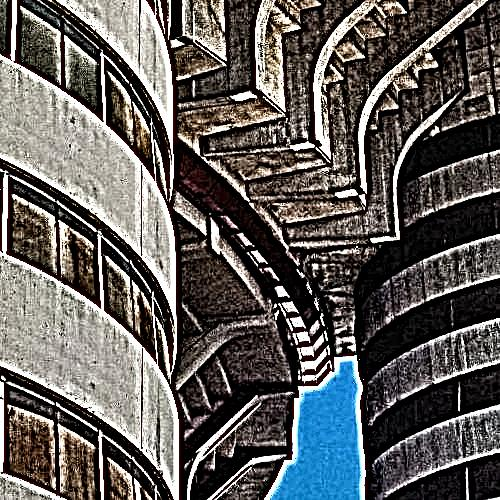
\includegraphics[width=\textwidth]{img/Sharpness.jpg}
        \caption{Sharpness}
        \label{fig:sharpness}
    \end{subfigure}
    \hfill
    \begin{subfigure}[b]{0.24\textwidth}
        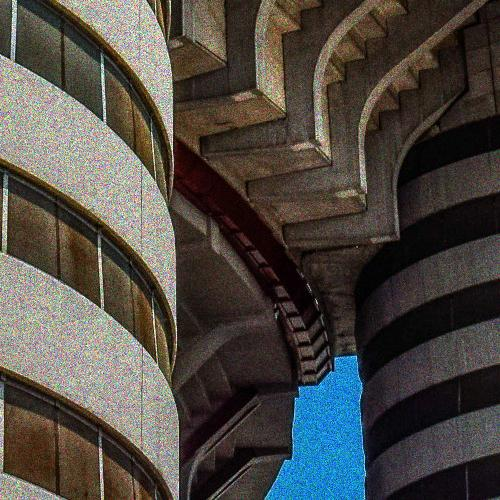
\includegraphics[width=\textwidth]{img/Noise.jpg}
        \caption{Noise}
        \label{fig:noise}
    \end{subfigure} 

    \begin{subfigure}[b]{0.24\textwidth}
        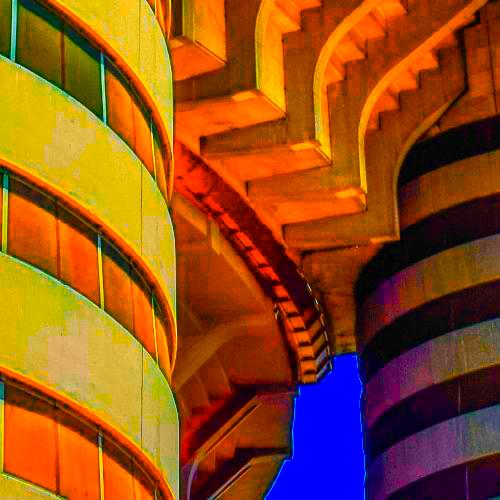
\includegraphics[width=\textwidth]{img/ColorAccuracy.jpg}
        \caption{Color Accuracy}
        \label{fig:color_accuracy}
    \end{subfigure}
    \hfill
    \begin{subfigure}[b]{0.24\textwidth}
        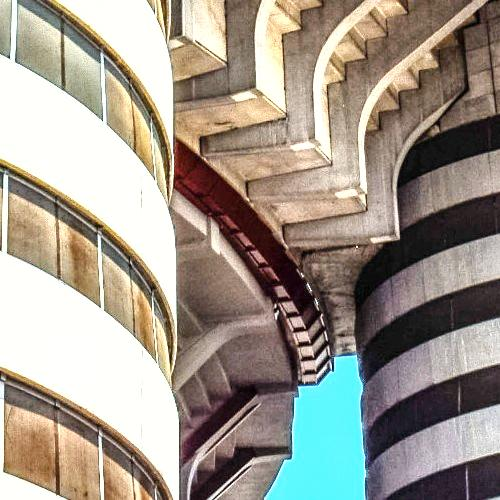
\includegraphics[width=\textwidth]{img/BrightnessContrast.jpg}
        \caption{Brightness \& Contrast}
        \label{fig:brightness_contrast}
    \end{subfigure}
    \hfill
    \begin{subfigure}[b]{0.24\textwidth}
        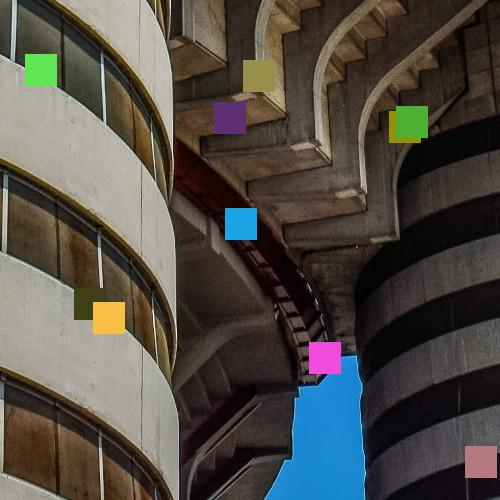
\includegraphics[width=\textwidth]{img/Artifacts.jpg}
        \caption{Artifacts}
        \label{fig:artifacts}
    \end{subfigure}
    \hfill
    \begin{subfigure}[b]{0.24\textwidth}
        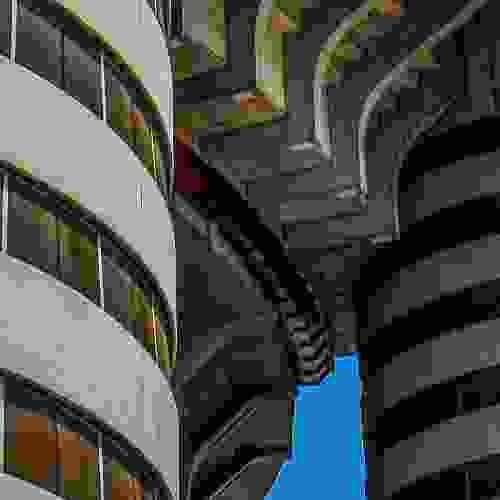
\includegraphics[width=\textwidth]{img/Compression.jpg}
        \caption{Compression}
        \label{fig:compression}
    \end{subfigure}
    \caption{Examples of Common Distortions in Images. (adapted from \autocite{ARNIQA})}
    \label{fig:distortions}
\end{figure}
\begin{enumerate}
    \item \textbf{Blur}: Blurred images lack sharpness and clarity, often resulting from motion during capturing, incorrect focus settings, or imperfections in the camera lens. See \autoref{fig:blur} for an example of a blurred image.
    \item \textbf{Sharpness}: Sharpness refers to how well-defined the edges and fine details in an image appear. High sharpness indicates clear, crisp images, while low sharpness makes an image look soft and unclear. See \autoref{fig:sharpness} for an example of a sharpened image.
    \item \textbf{Noise}: Noise appears as random variations in brightness or color and is often due to the limitations of the camera’s sensor, particularly under low light conditions or at high ISO settings. See \autoref{fig:noise} for an example of a noisy image.
    \item \textbf{Color Accuracy}:  Color accuracy refers to how faithfully colors are reproduced in an image. Distortions in color accuracy can lead to inaccurate or unrealistic color representation. See \autoref{fig:color_accuracy} for an example of a color-distorted image.
    \item \textbf{Brightness \& Contrast}: Brightness is the overall light level of an image, while contrast refers to the range between its darkest and lightest areas. Proper balance of both is crucial for maintaining image visibility and detail. Excessive or insufficient brightness and contrast can make an image unusable for detailed analysis. See \autoref{fig:brightness_contrast} for an example of an image with altered brightness.
    \item \textbf{Artifacts}: Artifacts are unwanted visual anomalies introduced during image acquisition or processing, such as halos, or jagged edges. See \autoref{fig:artifacts} for an example of an image with artifacts.
    \item \textbf{Compression}: When images are compressed to reduce file size, this often results in lost detail and visible quality degradation. See \autoref{fig:compression} for an example of a compressed image.
\end{enumerate}
Each type of distortion affects the visual quality and perceived accuracy of images, influencing the effectiveness of IQA methodologies in assessing image quality. Understanding these distortions is essential for developing robust quality assessment algorithms and improving image clarity in various applications, including teledermatology. \par

\subsection{Benchmark Datasets for IQA}
\label{sub:BenchmarkDatasetsIQA}
Benchmark datasets play a vital role in advancing Image Quality Assessment (IQA). They provide standardized and diverse image sets with known distortions and corresponding quality annotations, helping researchers evaluate and improve IQA algorithms. These annotations, often in the form of Mean Opinion Score (MOS) and Differential Mean Opinion Score (DMOS), serve as benchmarks for algorithm performance. \par
\vspace{\baselineskip}
\noindent
\textbf{Mean Opinion Score (MOS)} is calculated by averaging ratings from human observers who judge the quality of images on a predefined scale. This score reflects the overall perceptual quality as seen by typical viewers and is widely used to compare the performance of different IQA methods against human visual judgment. \par
\vspace{\baselineskip}
\noindent
\textbf{Differential Mean Opinion Score (DMOS)}, on the other hand, is derived from MOS and measures the perceived difference in quality between a reference image and a distorted version. This score is particularly useful for understanding the impact of specific distortions on image quality. \par
\vspace{\baselineskip}
\noindent
These datasets enable researchers to thoroughly test the robustness, accuracy, and generalization capabilities of different IQA methods. They also help in developing new algorithms by providing reliable quality scores, which are essential for ensuring reproducible. \par
\noindent
An overview of IQA databases is provided in \autoref{tab:iqa_databases}, and more detailed descriptions can be found in \autoref{ch:Dataset}.

\begin{table*}[!t]
    \centering
    \caption{An overview of IQA databases}
    \label{tab:iqa_databases}
    \renewcommand{\arraystretch}{1.5}
    \resizebox{\textwidth}{!}{ % Resize table to fit within the text width
    \begin{tabular}{p{2.3cm} p{2cm} c c c p{3.5cm} c  p{2.3cm} c}
    \toprule
        Category & Database & Year & \#Ref. & \#Dist. & \#Dist. Type & \#Dist. Level & Resolution Type & Ground-truth \\
        \hline
        \multirow{8}{*}{General} 
        & LIVE & 2004 & 30 & 779 & JPEG, JP2K, WN, GB, FF& 5 or 4 & 768 $\times$ 512 & DMOS \\
        & TID2008 & 2008 & 25 & 1700 & 17 \footnote{See detailed types on database page: \url{https://www.ponomarenko.info/tid2008.htm}} & 4 & 512 $\times$ 384 & MOS \\
        & TID2013 & 2013 & 25 & 3000 & 24 \footnote{See detailed types on database page: \url{https://www.ponomarenko.info/tid2013.htm}} & 5 & 512 $\times$ 384 & MOS \\
        & CSIQ & 2009 & 30 & 866 & JPEG, JP2K, WN, GB, APGN,  GCD & 5 or 4 & 512 $\times$ 512 & DMOS \\
        & A57 & 2007 & 3 & 54 & DWT, AGWN, JPEG, JP2K, JP2K-DCQ, GB& 3 & 512 $\times$ 512 & MOS \\
        & WED & 2017 & 4744 & 94880 & JPEG, JP2K, GB, WN& 5 & - & - \\
        & KADID-10k & 2019& 81& 10125& 25 \footnote{See detailed types on database page: \url{https://database.mmsp-kn.de/kadid-10k-database.html}} & 5& 512 $\times$ 384 & DMOS\\
        & KADIS-700k & 2020& 140000& 700000& 25 \footnote{See detailed types on database page: \url{https://database.mmsp-kn.de/kadid-10k-database.html}} & 5& 512 $\times$ 384 & DMOS\\
        \hline
        \multirow{3}{*}{Multiple Dist.} 
        & LIVEMD & 2012 & 15 & 405 & GB followed by JPEG, GB followed by WN& - & 1280 $\times$ 720 & DMOS \\
        & MDID2013 & 2013 & 12 & 324 & corrupted successively by GB, WN, and JPEG& - & 768 $\times$ 512 or 1280 $\times$ 720 & DMOS \\
        & MDID2016 & 2016 & 20 & 1600 & GB or CC first, JPEG or JP2K second and WN last& - & 512 $\times$ 384 & MOS \\
        \hline
        \multirow{4}{*}{Screen content} 
        & SIQAD & 2014 & 20 & 980 & WN, GB, CC, JPEG, JP2K, MB, LSBC& 7 & 700 $\times$ 700 & DMOS \\
        & SCIQ & 2017 & 40 & 1800 & WN, GB, MB, CC, JPEG, JP2K, CSC, CQD& 5 & 1280 $\times$ 720 & MOS \\
        & CCT & 2017 & 72 & 1320 & HEVC and HEVC-SCC coding& 11 & 1280 $\times$ 720 to 1920 $\times$ 1080 & MOS \\
        & HSNID & 2019 & 20 & 600 & WN, GB, MB, CC, JPEG, JP2K& 5 &  - & MOS \\
        \hline
        \multirow{2}{*}{Authentic Dist.} 
        & LIVE Wild & 2016 & 0 & 1162 & - & - & 500 $\times$ 500 & MOS \\
        & CID2013 & 2015 & 0 & 480 & - & - & 1600 $\times$ 1200 & MOS \\
    \bottomrule
    \end{tabular}
    }
    \raggedright
    \scalebox{0.59}{
    \begin{tabular}{l}
        Note: \#Ref.: Total number of pristine images. \quad \#Dist.: Total number of distorted images. \quad AGWN: Additive Gaussian white noise. \quad WN: White noise.\\
        \quad  \quad  \quad APGN: Additive pink Gaussian noise. \quad CC: Contrast change. \quad CSC: Color saturation change. \quad CQD: Color quantization with dithering.\\
        \quad  \quad  \quad DWT: Quantization of the LH subbands of a 5-level DWT. \quad FF: Simulated fast fading Rayleigh channel. \quad GB: Gaussian blur. \quad MB: Motion blur.\\
        \quad  \quad  \quad GCD: Global contrast decrements. \quad HEVC-SCC: Screen content coding extension of high efficiency video coding. \quad JPEG: JPEG compression. \\
        \quad  \quad  \quad JP2K: JPEG2000 compression. \quad JP2K-DCQ: JPEG-2000 compression with DCQ. \quad LSBC: Layer segmentation based compression.
    \end{tabular}
    }
\end{table*}


\subsection{State-of-the-Art in Image Quality Assessment}
\label{sub:SOTA_IQA}
The current state-of-the-art in Image Quality Assessment (IQA) is ARNIQA \autocite{ARNIQA} , with version 2 released on November 4, 2023. ARNIQA (leArning distoRtion maNifold for Image Quality Assessment) represents a major advancement in No-Reference Image Quality Assessment (NR-IQA). This technology aims to measure image quality based on human perception, even without a reference image. This capability is crucial in fields like teledermatology, where the quality of images directly impacts diagnostic accuracy. \par
\vspace{\baselineskip}
\noindent
\textbf{Overview of ARNIQA}: ARNIQA is developed using a self-supervised learning approach. It learns a comprehensive model of all possible image distortions, focusing on the types and quality of distortions rather than the content of the images themselves. This makes it highly adaptable across various domains where image content can differ significantly. \par
\vspace{\baselineskip}
\noindent
\textbf{Key Features of ARNIQA}:
\begin{enumerate}
    \item Image Degradation Model: ARNIQA can synthetically degrade images through up to 1.9 billion distinct degradation patterns. This model can apply up to seven different types of distortions in one sequence, covering a wide range of real-world scenarios. Training with such diverse distortions ensures that ARNIQA can accurately assess image quality across various conditions and avoid the need for large labeled datasets.
    \item SimCLR Framework: At the core of ARNIQA is the SimCLR (Simple Framework for Contrastive Learning) framework. This framework enables the model to learn meaningful representations of image quality by comparing different versions of the same image and focusing on their similarities and differences. SimCLR constructs positive pairs by applying the same distortion settings to two different images, ensuring that the model concentrates on the distortions rather than the content. To further enhance the model’s discriminative capability, SimCLR introduces subtle variations by downsampling images before cropping and applying distortions, creating hard negative examples. These examples help the model differentiate between similar-looking images with different types of degradation. By using this approach, the SimCLR framework ensures that ARNIQA effectively learns to recognize and assess various distortions, enhancing its ability to provide accurate image quality assessments (see \autoref{fig:SimCLR}).
    \item Linear Regressor: A Linear Regressor maps the features learned by SimCLR to qualtiy score ranging from 0 to 1. This score reflects the relative quality of the image based on the distortions present.
\end{enumerate}
\vspace{\baselineskip}
\noindent
\textbf{Training Strategy of ARNIQA}: ARNIQA’s training strategy involves two main phases: \par
\begin{enumerate}
    \item Encoder Pre-training: The model is first trained on a large set of unlabeled images that are synthetically degraded. This helps the encoder learn features related to different types and levels of image degradation.
    \item Regressor Training:In the second phase, a specific regressor is trained using the Mean Opinion Scores (MOS) of images. This step translates the learned features into actual quality scores.
\end{enumerate}
\vspace{\baselineskip}
\noindent
\textbf{Advantages of ARNIQA}: ARNIQA achieves high performance with only up to 0.5\% of the data required by other methods, thanks to its focus on distortion patterns rather than image content. It provides reliable and consistent quality assessments across a wide range of distortions and severities, demonstrating its robustness. Additionally, ARNIQA is particularly suitable for teledermatology as it can handle varying image quality resulting from different lighting conditions, camera quality, and patient handling. \par
\begin{figure}[ht]
    \centering
    
\includegraphics[keepaspectratio,width=15cm]{img/method_SimCLR.jpg}
    \caption{Overview of the training strategy for ARNIQA. Two pristine images are cropped and equally degraded. The model maximizes the similarity of their embeddings while minimizing the similarity to embeddings from degraded crops of half-scale versions of the original images. This process creates hard negative examples by introducing downsample distortion, demonstrating how original and half-scale degraded crops differ despite identical degradation. \autocite{ARNIQA}.}
    \label{fig:SimCLR}
\end{figure}

\subsection{Challenges and Opportunities in Image Quality Assessment}
\label{sub:ChallengesOpportunitiesIQA}
In the realm of Image Quality Assessment (IQA), practitioners face the challenge of accounting for the variability of conditions under which images are captured. This is especially true in teledermatology, where variables such as lighting and camera quality can significantly affect image consistency. Moreover, the subjectivity inherent in human visual perception adds complexity to developing algorithms that accurately reflect human assessments of image quality.\par
\vspace{\baselineskip}
\noindent
Another significant challenge is the diversity of image content, which makes it difficult to apply uniform quality criteria across different types of images. Additionally, real-world images often present multiple interacting distortions, unlike the isolated distortions typically studied in laboratory settings, complicating the quality assessment process. Scalability also presents a hurdle, as the increasing volume of image data demands efficient processing for quality evaluation.\par
\vspace{\baselineskip}
\noindent
On the other side, the landscape of IQA also presents several opportunities. Advances in machine learning, particularly with self-supervised approaches like ARNIQA, open up new possibilities for training models that require less annotated data and can generalize across various conditions. Such technological progress bodes well for teledermatology, where enhanced IQA could lead to more accurate diagnoses.\par
\vspace{\baselineskip}
\noindent
The drive towards standardized image capturing and processing protocols represents another opportunity to improve image quality consistency. Additionally, interdisciplinary research combining insights from computer science, imaging, and medical fields is essential to tailor IQA methods for specific medical applications. Finally, leveraging big data analytics can provide a comprehensive understanding of common quality issues, informing the development of more refined IQA tools. \par


\section{Teledermatology}
\label{sec:Teledermatology}
Within the dynamic spectrum of telemedicine, teledermatology emerges as a distinct application that utilizes information and communication technologies to facilitate dermatological consultations remotely. This modality of healthcare has seen widespread adoption, especially in resource-rich regions like Europe and North America, where the availability of advanced technologies has allowed for the provision of high-quality images essential for accurate diagnoses. \par

The following section provides an overview of teledermatology, a specialized field of dermatology that utilizes telecommunications technology to provide remote diagnosis and consultation for skin conditions. This section discusses the importance of image quality in teledermatology, quality criteria for teledermatology images, as well as challenges and opportunities associated with the practice. \par
\vspace{\baselineskip}
\noindent

\subsection{Introduction to Teledermatology}
\label{sub:IntroductionTeledermatology}
Teledermatology can be effectively categorized into two primary approaches: real-time (RT) and store-and-forward (S\&F). RT teledermatology facilitates live interactions between patients and physicians through video calls, while S\&F involves capturing and sending images for later review by a dermatologist. The S\&F method has gained prominence due to its convenience and adaptability to varying schedules.\par
\vspace{\baselineskip}
\noindent
A typical teledermatology workflow begins with the patient capturing an image of their skin condition using a digital device. This image is then transmitted through a teledermatology platform to a medical expert who reviews the image's quality and details. The dermatologist then provides a report or prescription back to the patient, completing the consultation cycle. This workflow underscores the critical nature of image quality in teledermatology, as diagnostic accuracy is heavily reliant on the clarity and fidelity of the transmitted images.\par

\subsection{Importance of Image Quality in Teledermatology}
\label{sub:ImportanceIQA_Teledermatology}
In teledermatology, the caliber of transmitted images is critically pivotal. Clear and detailed images are the foundation upon which dermatologists rely for diagnosing and managing skin conditions from afar. When the images are of high quality, they capture essential details such as texture and color nuances that can be key to distinguishing between benign and more severe dermatological issues.\par
\vspace{\baselineskip}
\noindent

The resolution, focus, and accurate color representation in these images can markedly streamline the teledermatological process. They minimize the necessity for additional consultations due to poor image clarity, thereby improving the overall efficiency of the healthcare system and reducing patient wait times.\par
\vspace{\baselineskip}
\noindent

As the primary conduit for remote dermatological assessment, the images not only facilitate immediate patient care but also feed into the broader ecosystem of teledermatology that includes emerging technologies such as artificial intelligence. High-fidelity images are integral to training sophisticated AI algorithms, which promise to further enhance diagnostic precision and expedite the triage process.\par
\vspace{\baselineskip}
\noindent

In summary, the emphasis on image quality in teledermatology is not merely a current requirement but a crucial investment in the future of dermatological care, ensuring continued improvements in patient outcomes and the evolution of healthcare delivery methods.

\subsection{Quality Criteria for Teledermatology Images}
\label{sub:QualityCriteriaTeledermatology}
In teledermatology, the efficacy of remote diagnoses heavily relies on the quality of the images. Just as Image Quality Assessment (IQA) must confront various distortions affecting image perception, teledermatology faces its own set of quality criteria that are essential for effective practice. Proper lighting, background uniformity, appropriate field of view, accurate orientation, precise focus and depth of field, high resolution, and correct color calibration are paramount in ensuring that the dermatological images transmitted for evaluation are of the highest possible quality.
\begin{figure}[ht]
    \centering
    \begin{subfigure}[b]{0.24\textwidth}
        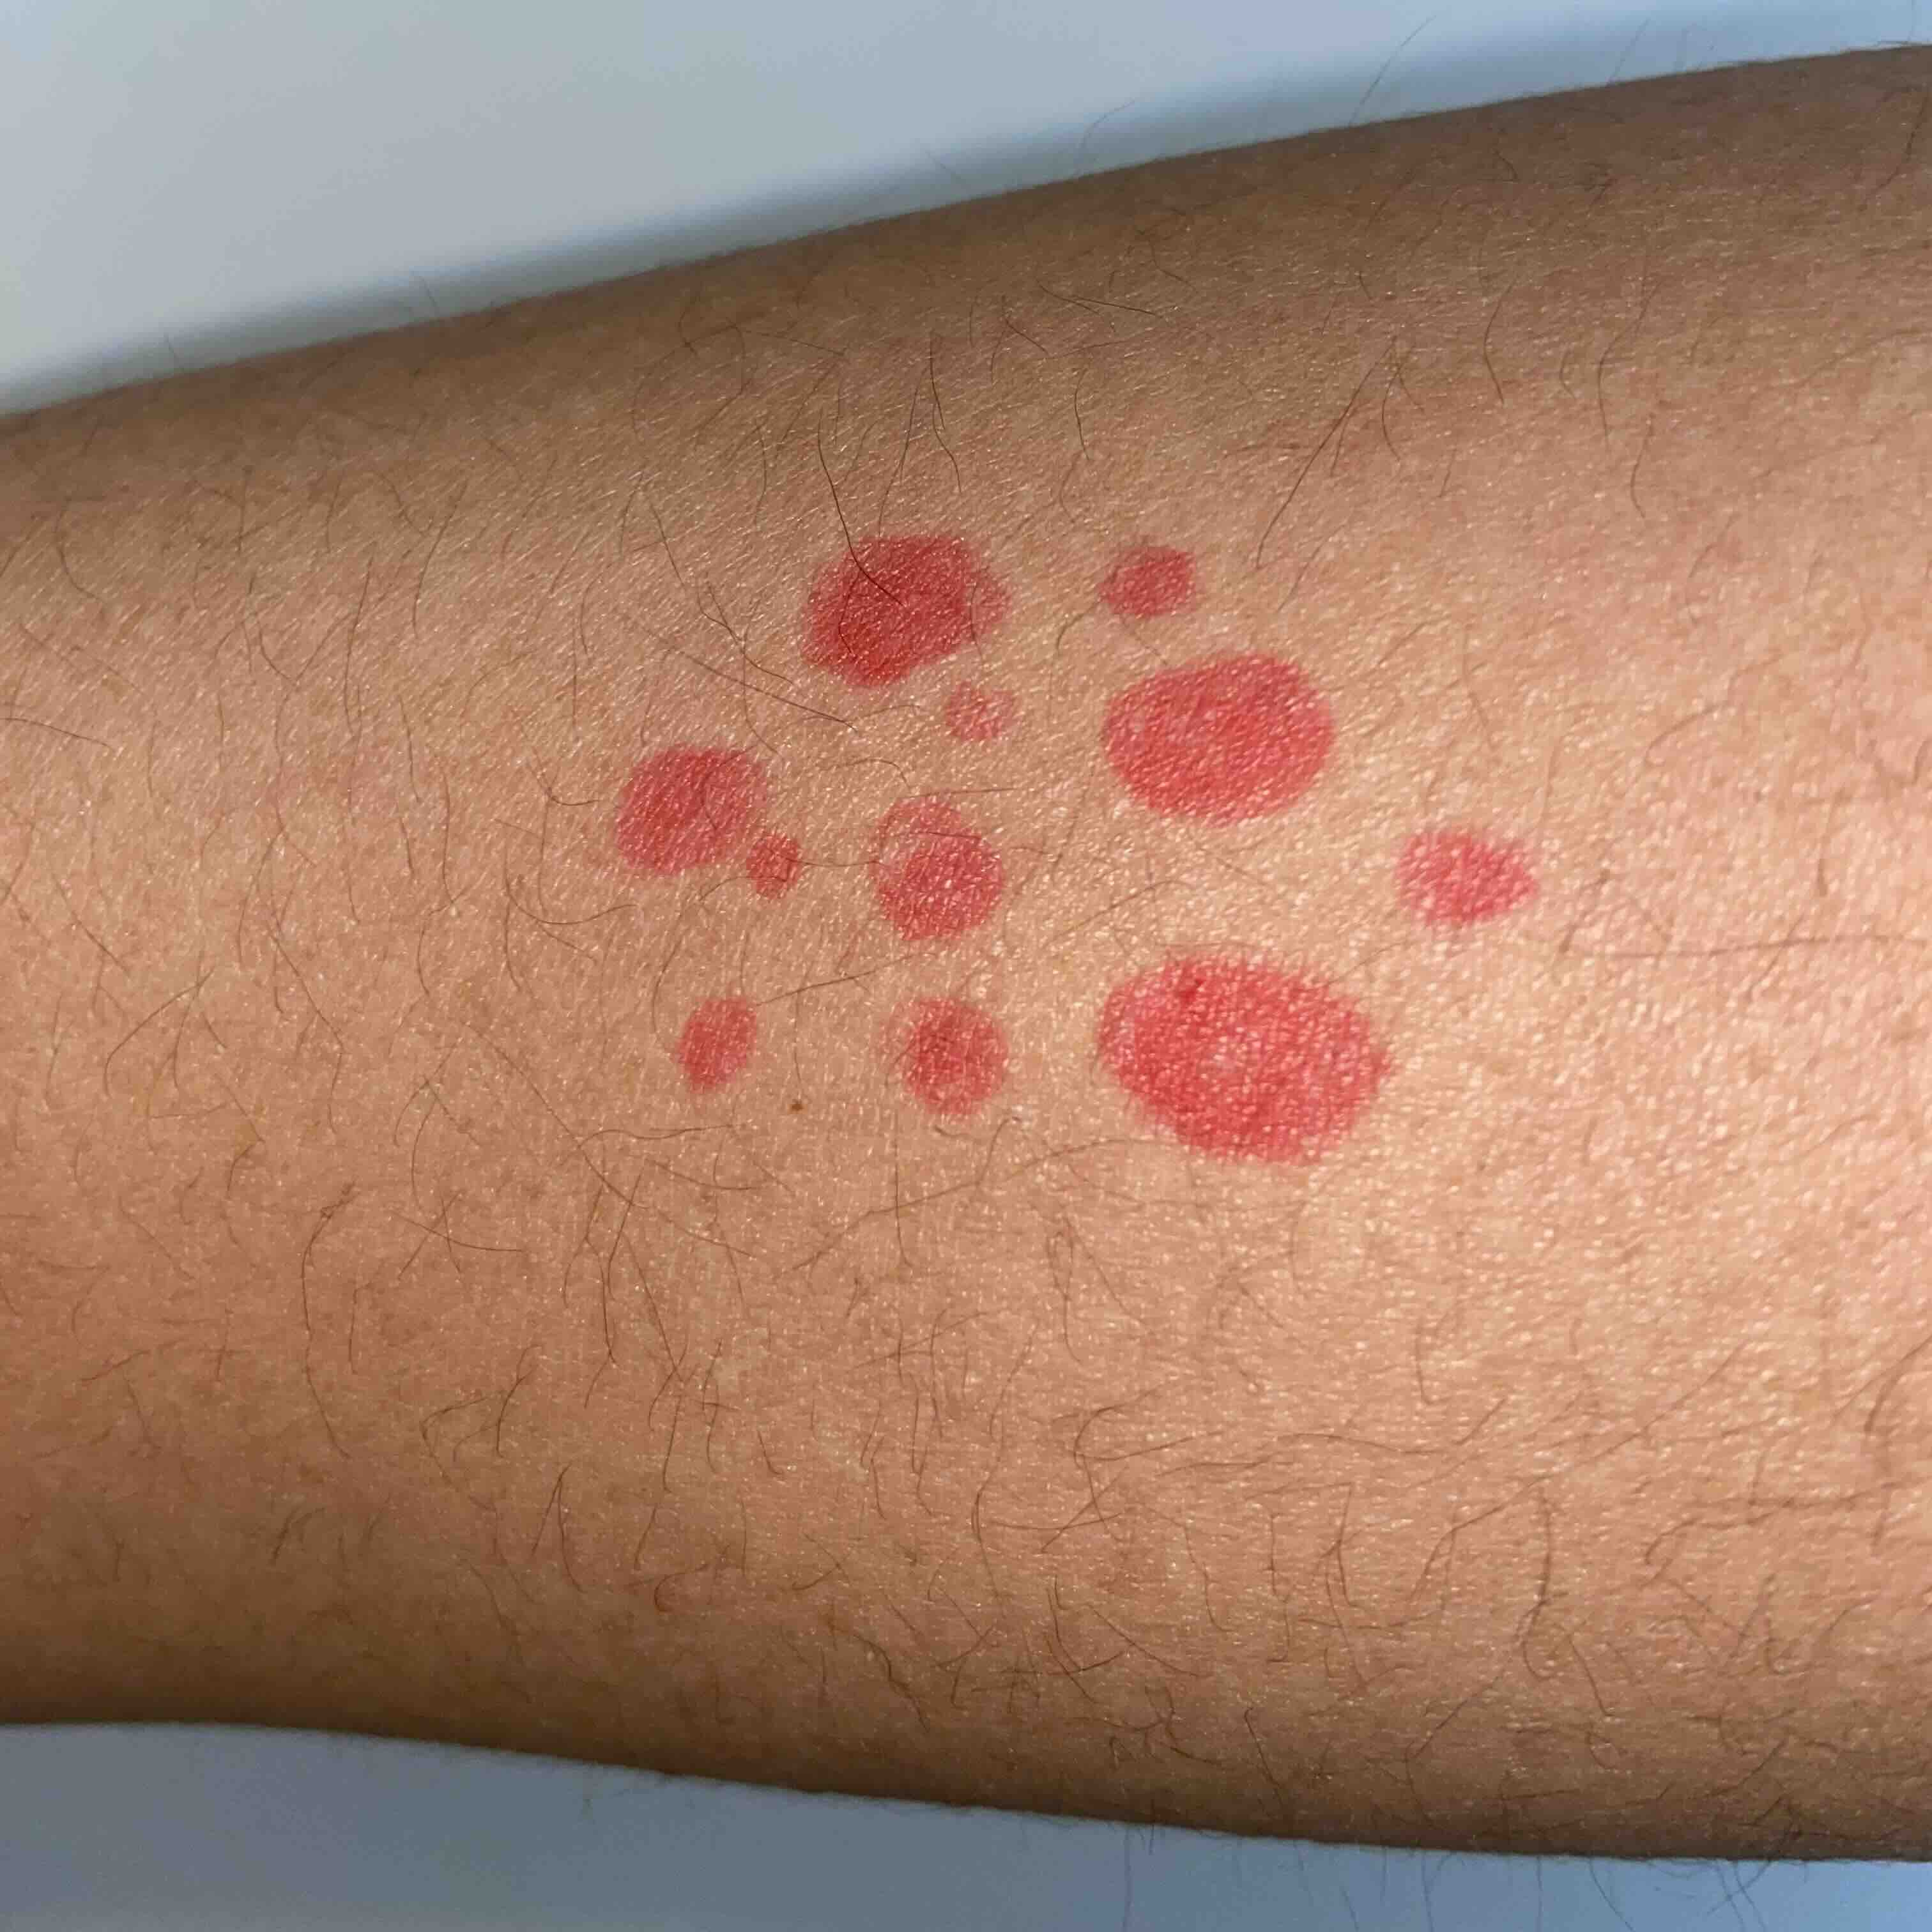
\includegraphics[width=\textwidth]{img/Reference.jpg}
        \caption{Good Quality}
    \end{subfigure}
    \hfill
    \begin{subfigure}[b]{0.24\textwidth}
        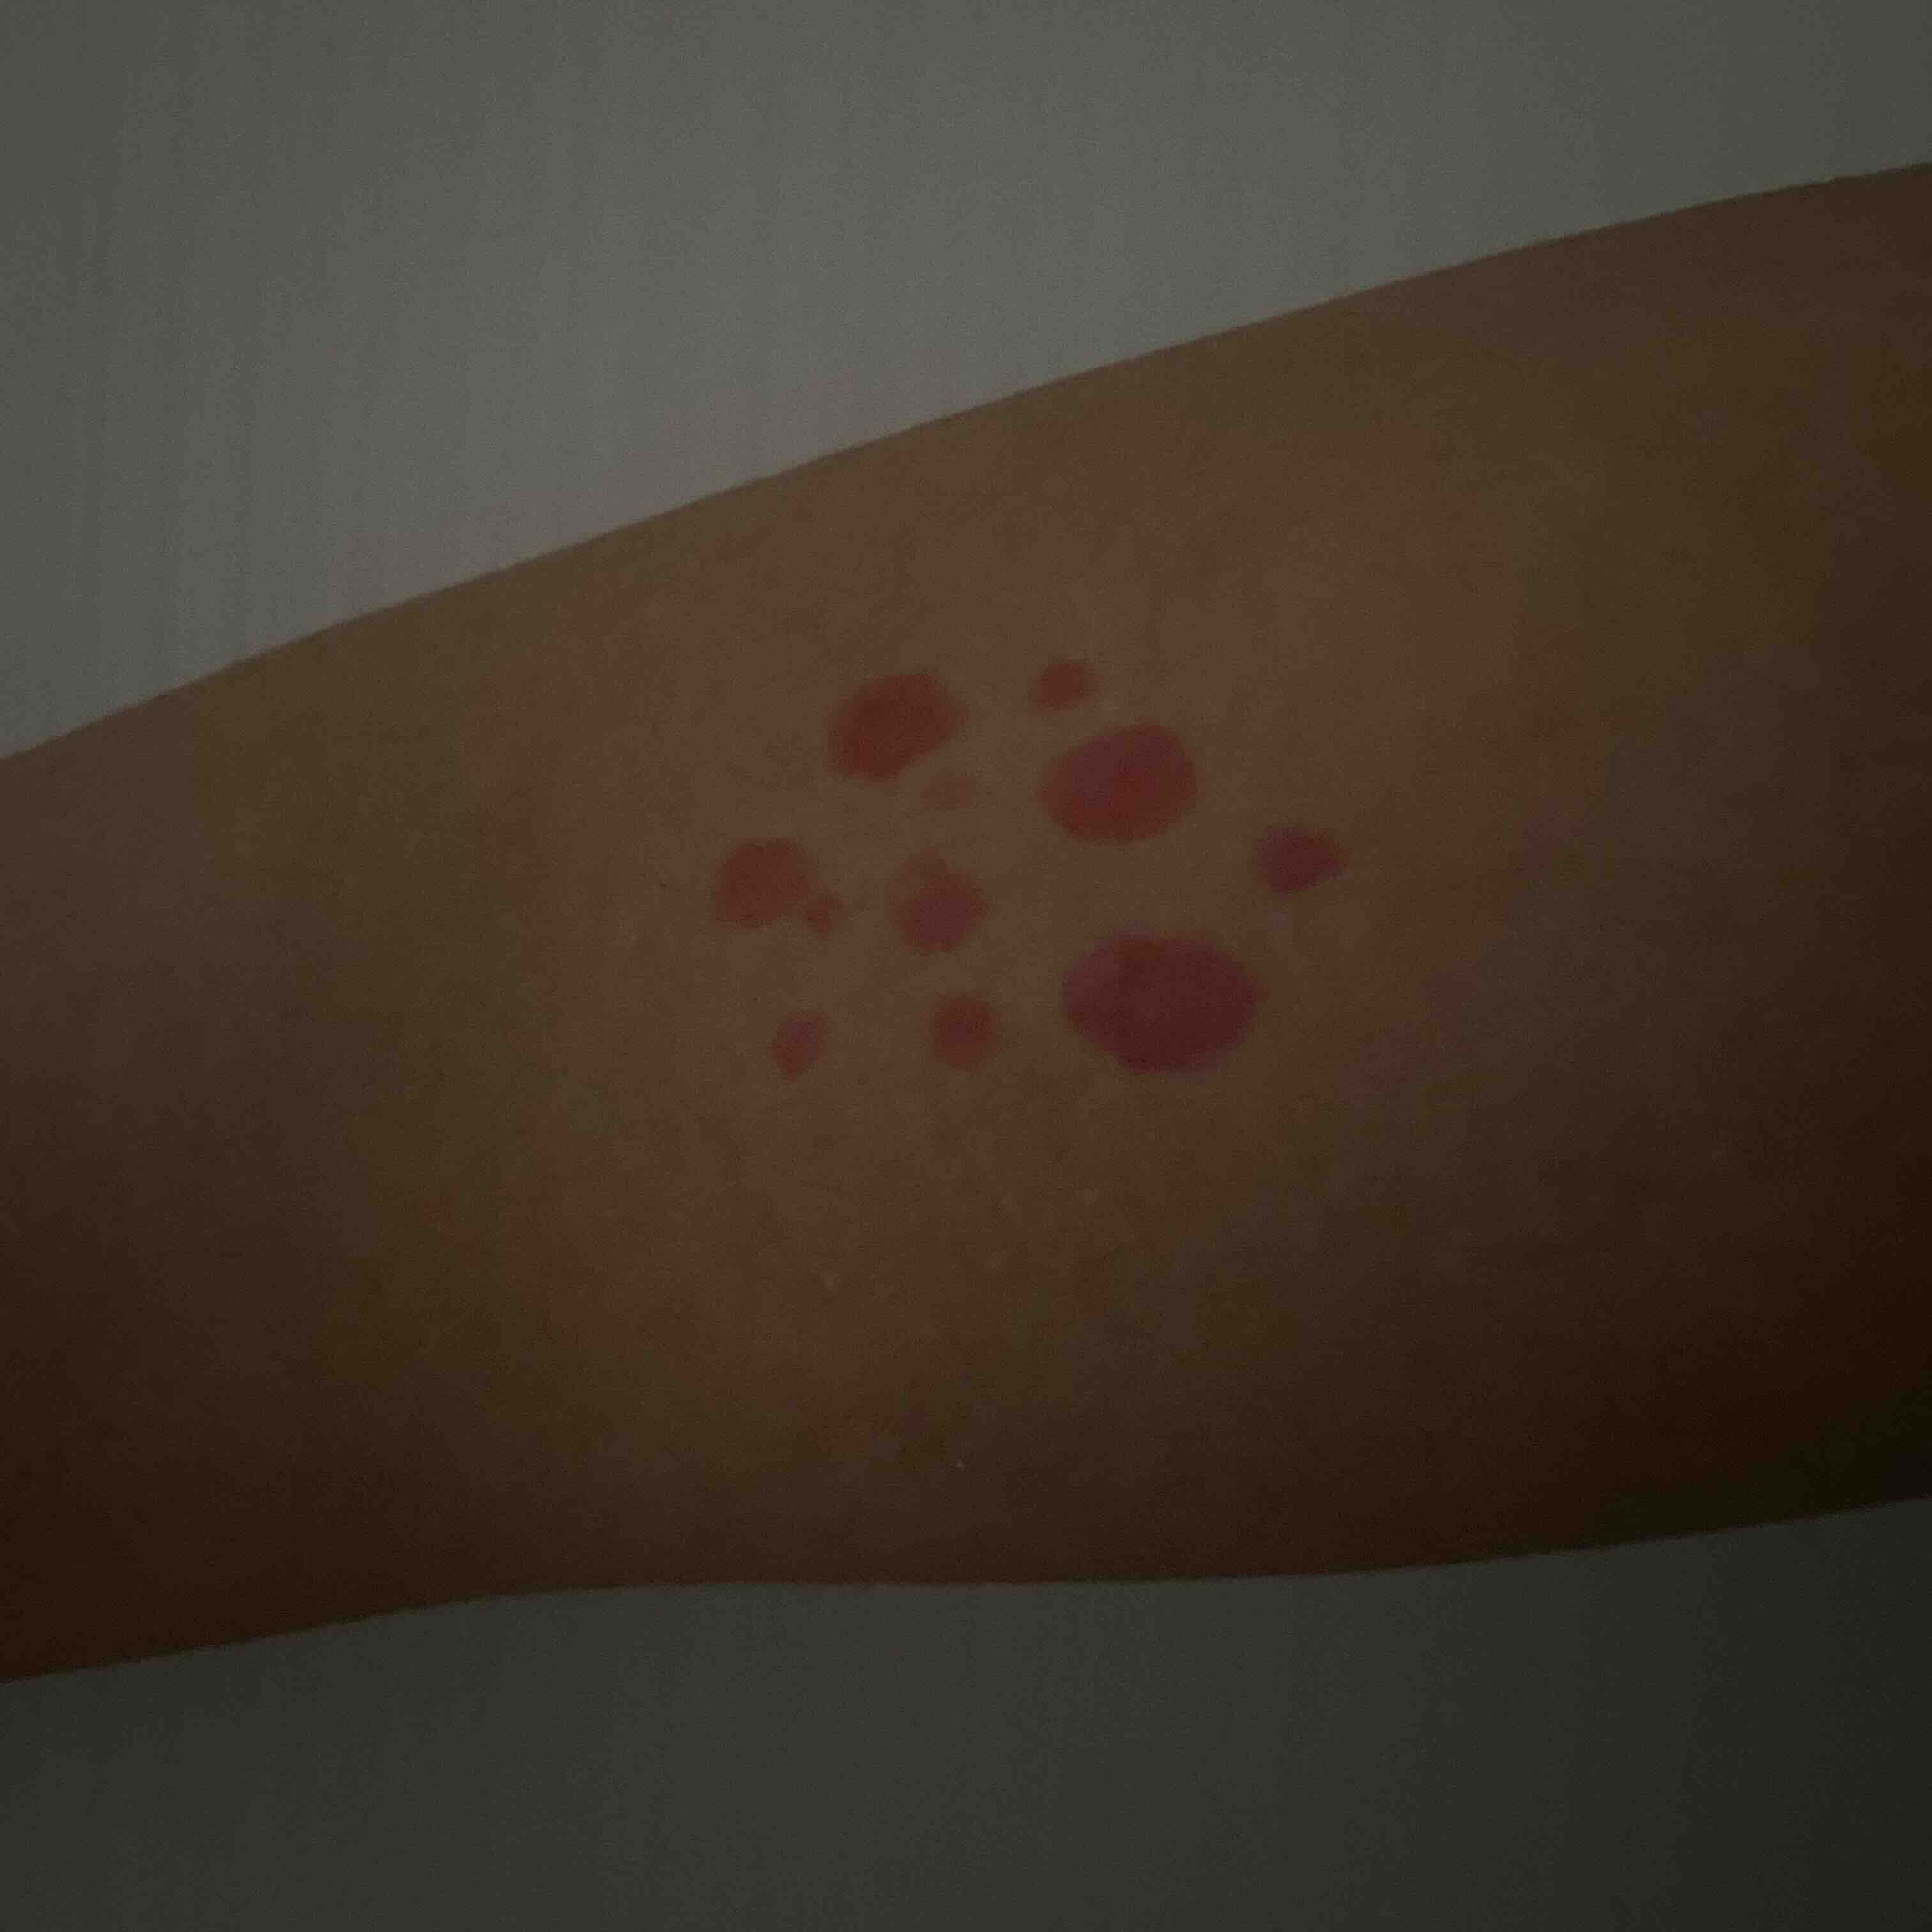
\includegraphics[width=\textwidth]{img/Lighting.jpg}
        \caption{Lighting}
        \label{fig:lighting}
    \end{subfigure}
    \hfill
    \begin{subfigure}[b]{0.24\textwidth}
        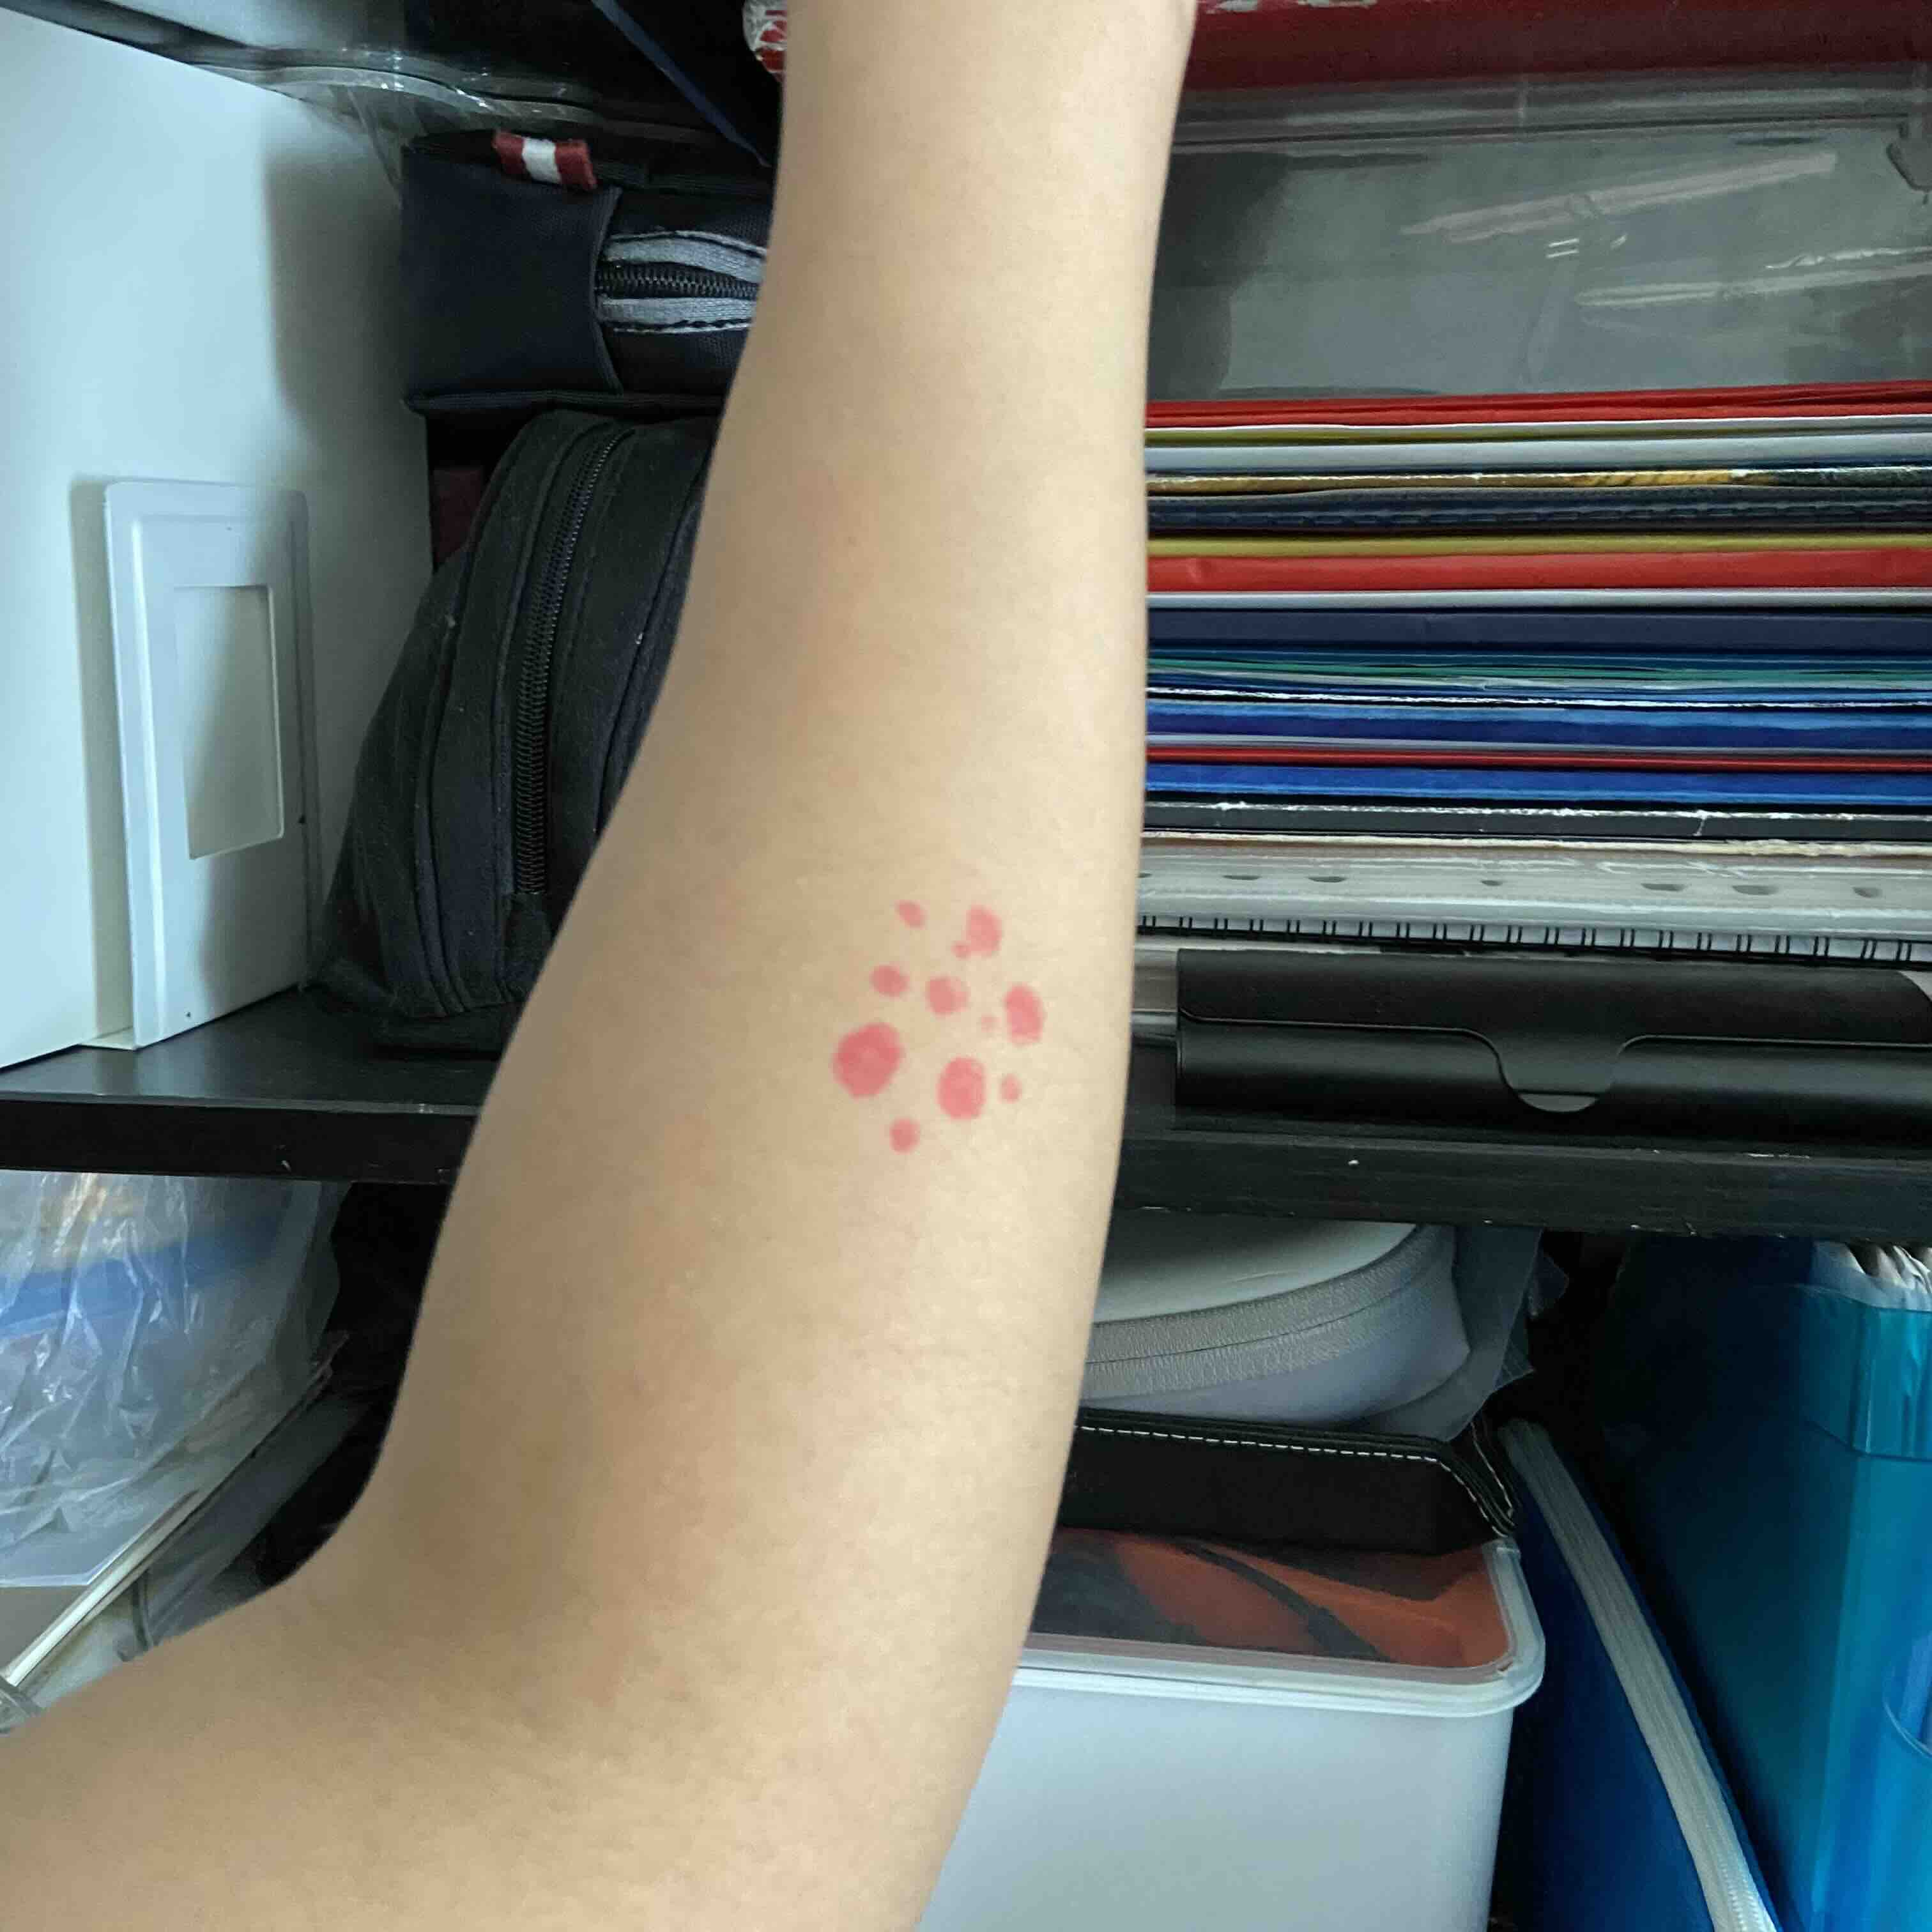
\includegraphics[width=\textwidth]{img/Background.jpg}
        \caption{Background}
        \label{fig:background}
    \end{subfigure}
    \hfill
    \begin{subfigure}[b]{0.24\textwidth}
        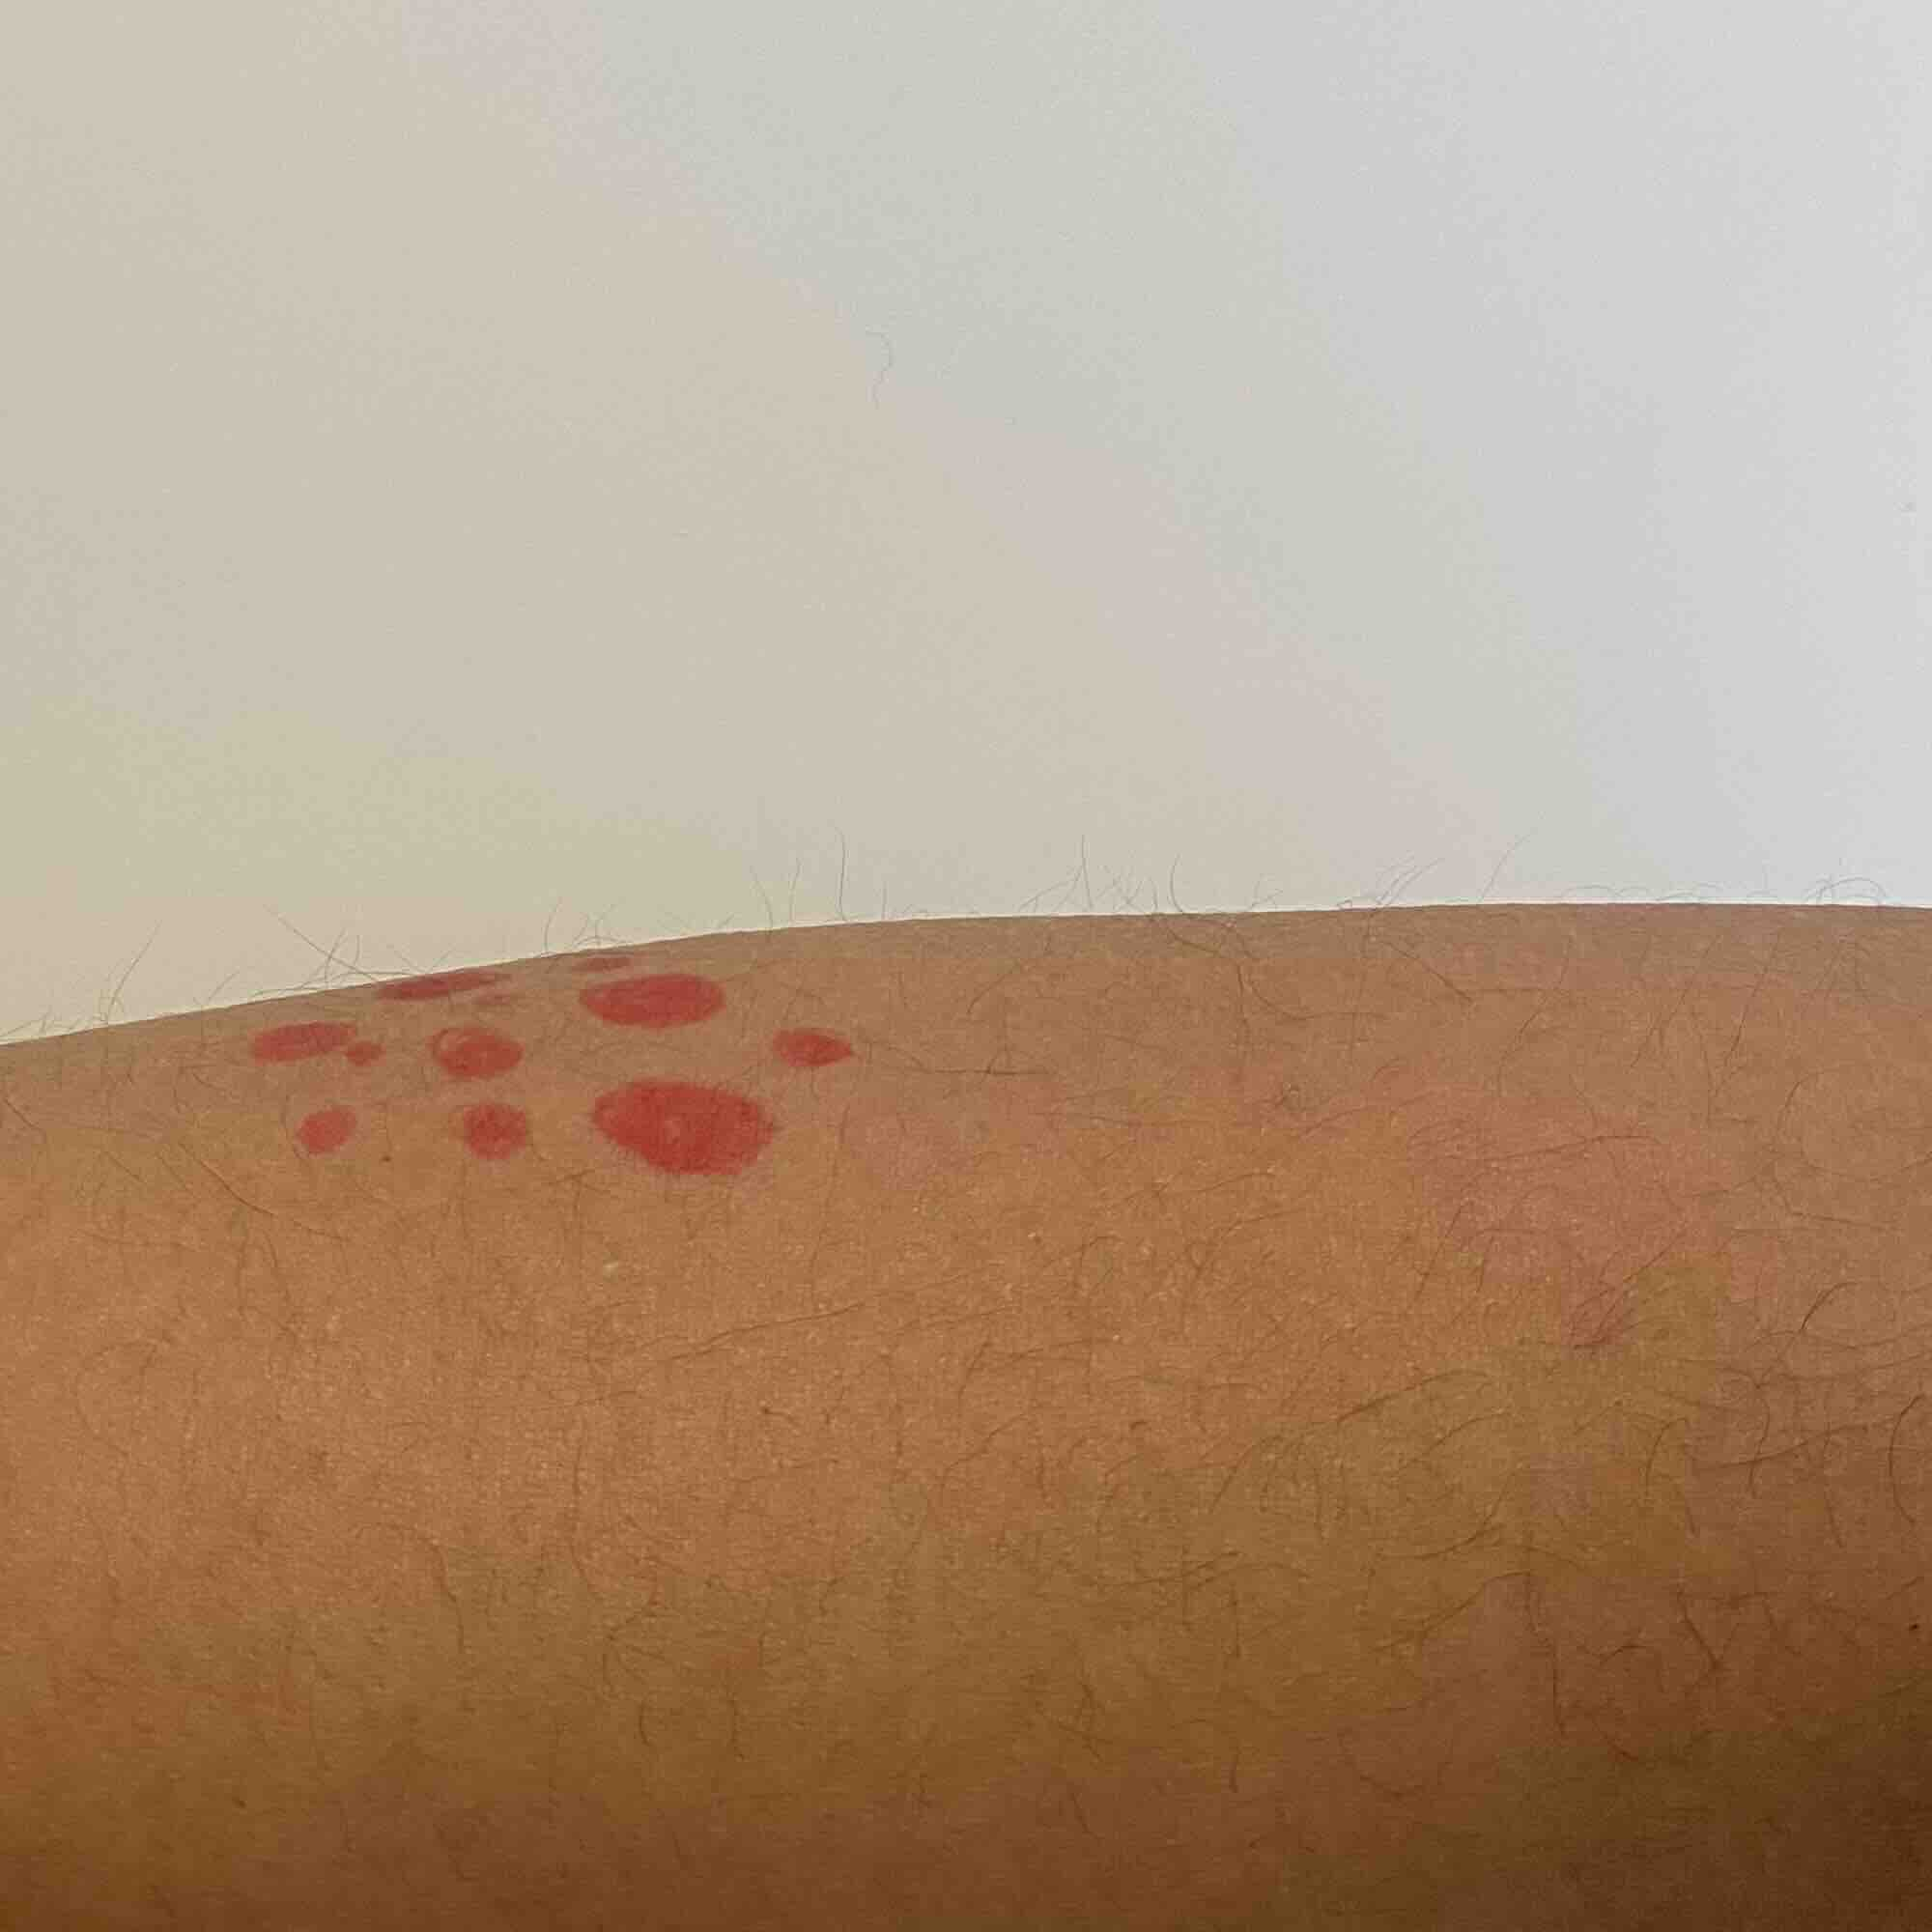
\includegraphics[width=\textwidth]{img/FoV.jpg}
        \caption{Field of View}
        \label{fig:FoV}
    \end{subfigure} 

    \begin{subfigure}[b]{0.24\textwidth}
        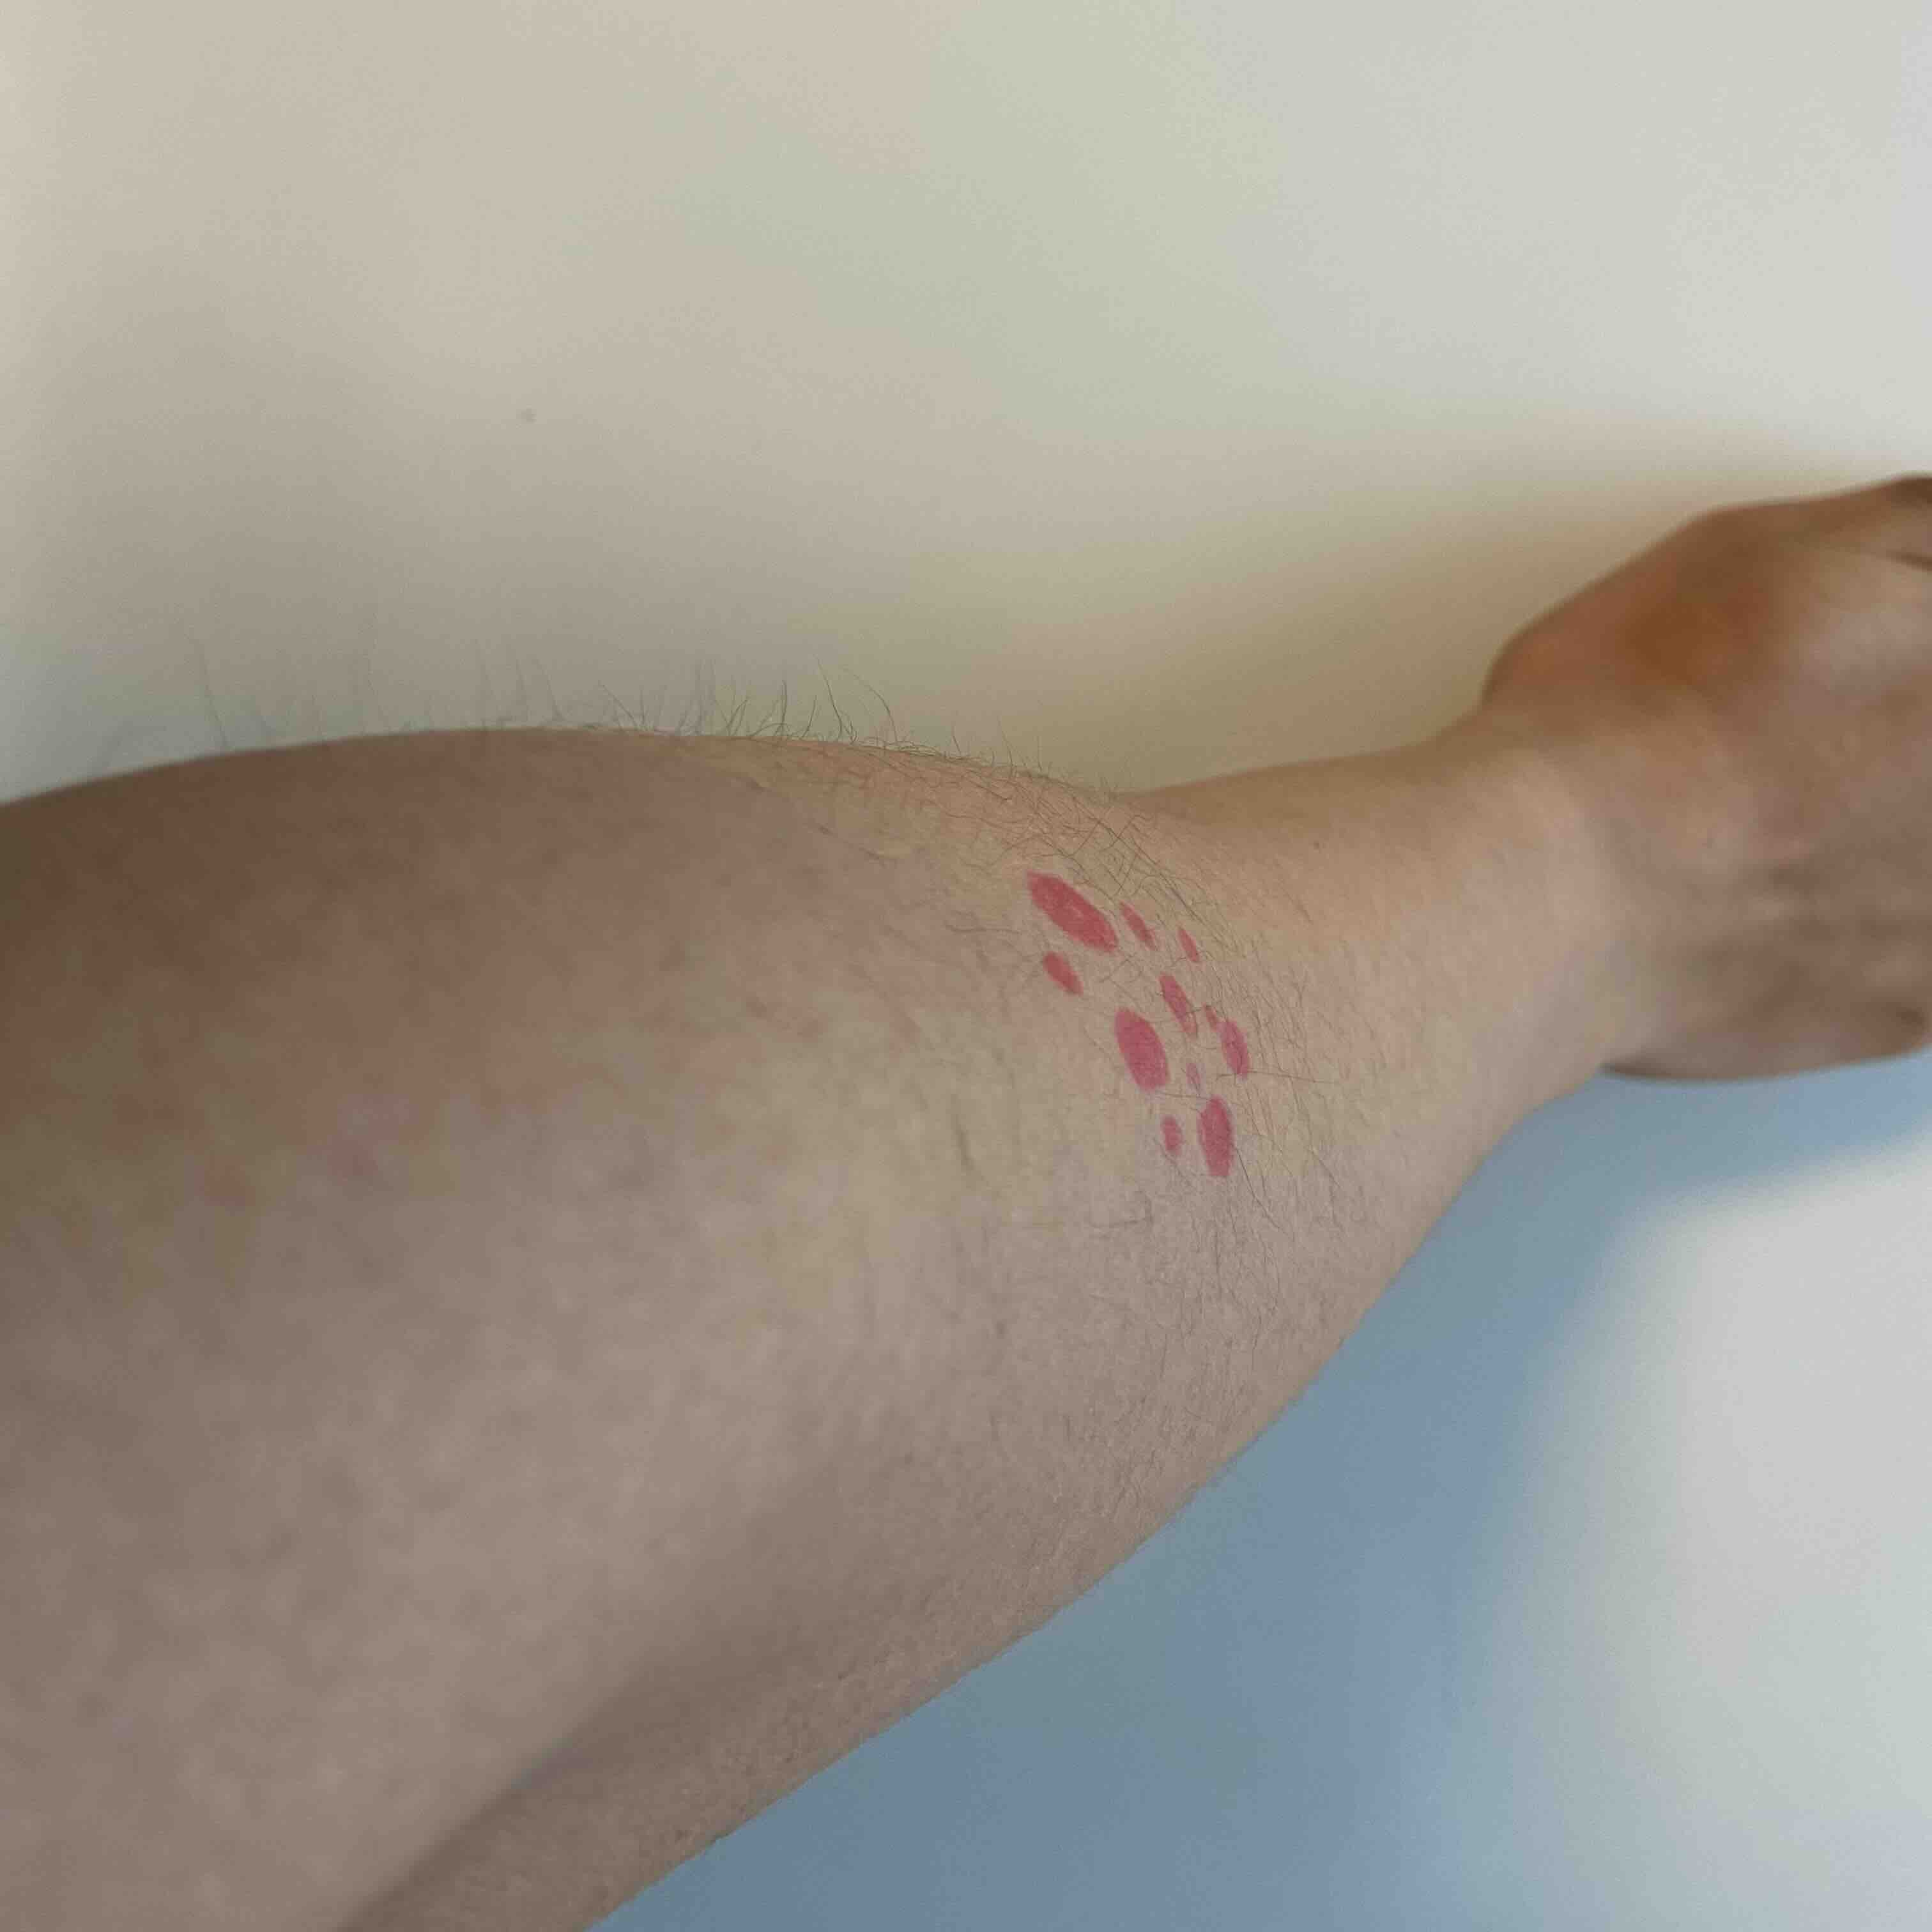
\includegraphics[width=\textwidth]{img/Orientation.jpg}
        \caption{Orientation}
        \label{fig:orientation}
    \end{subfigure}
    \hfill
    \begin{subfigure}[b]{0.24\textwidth}
        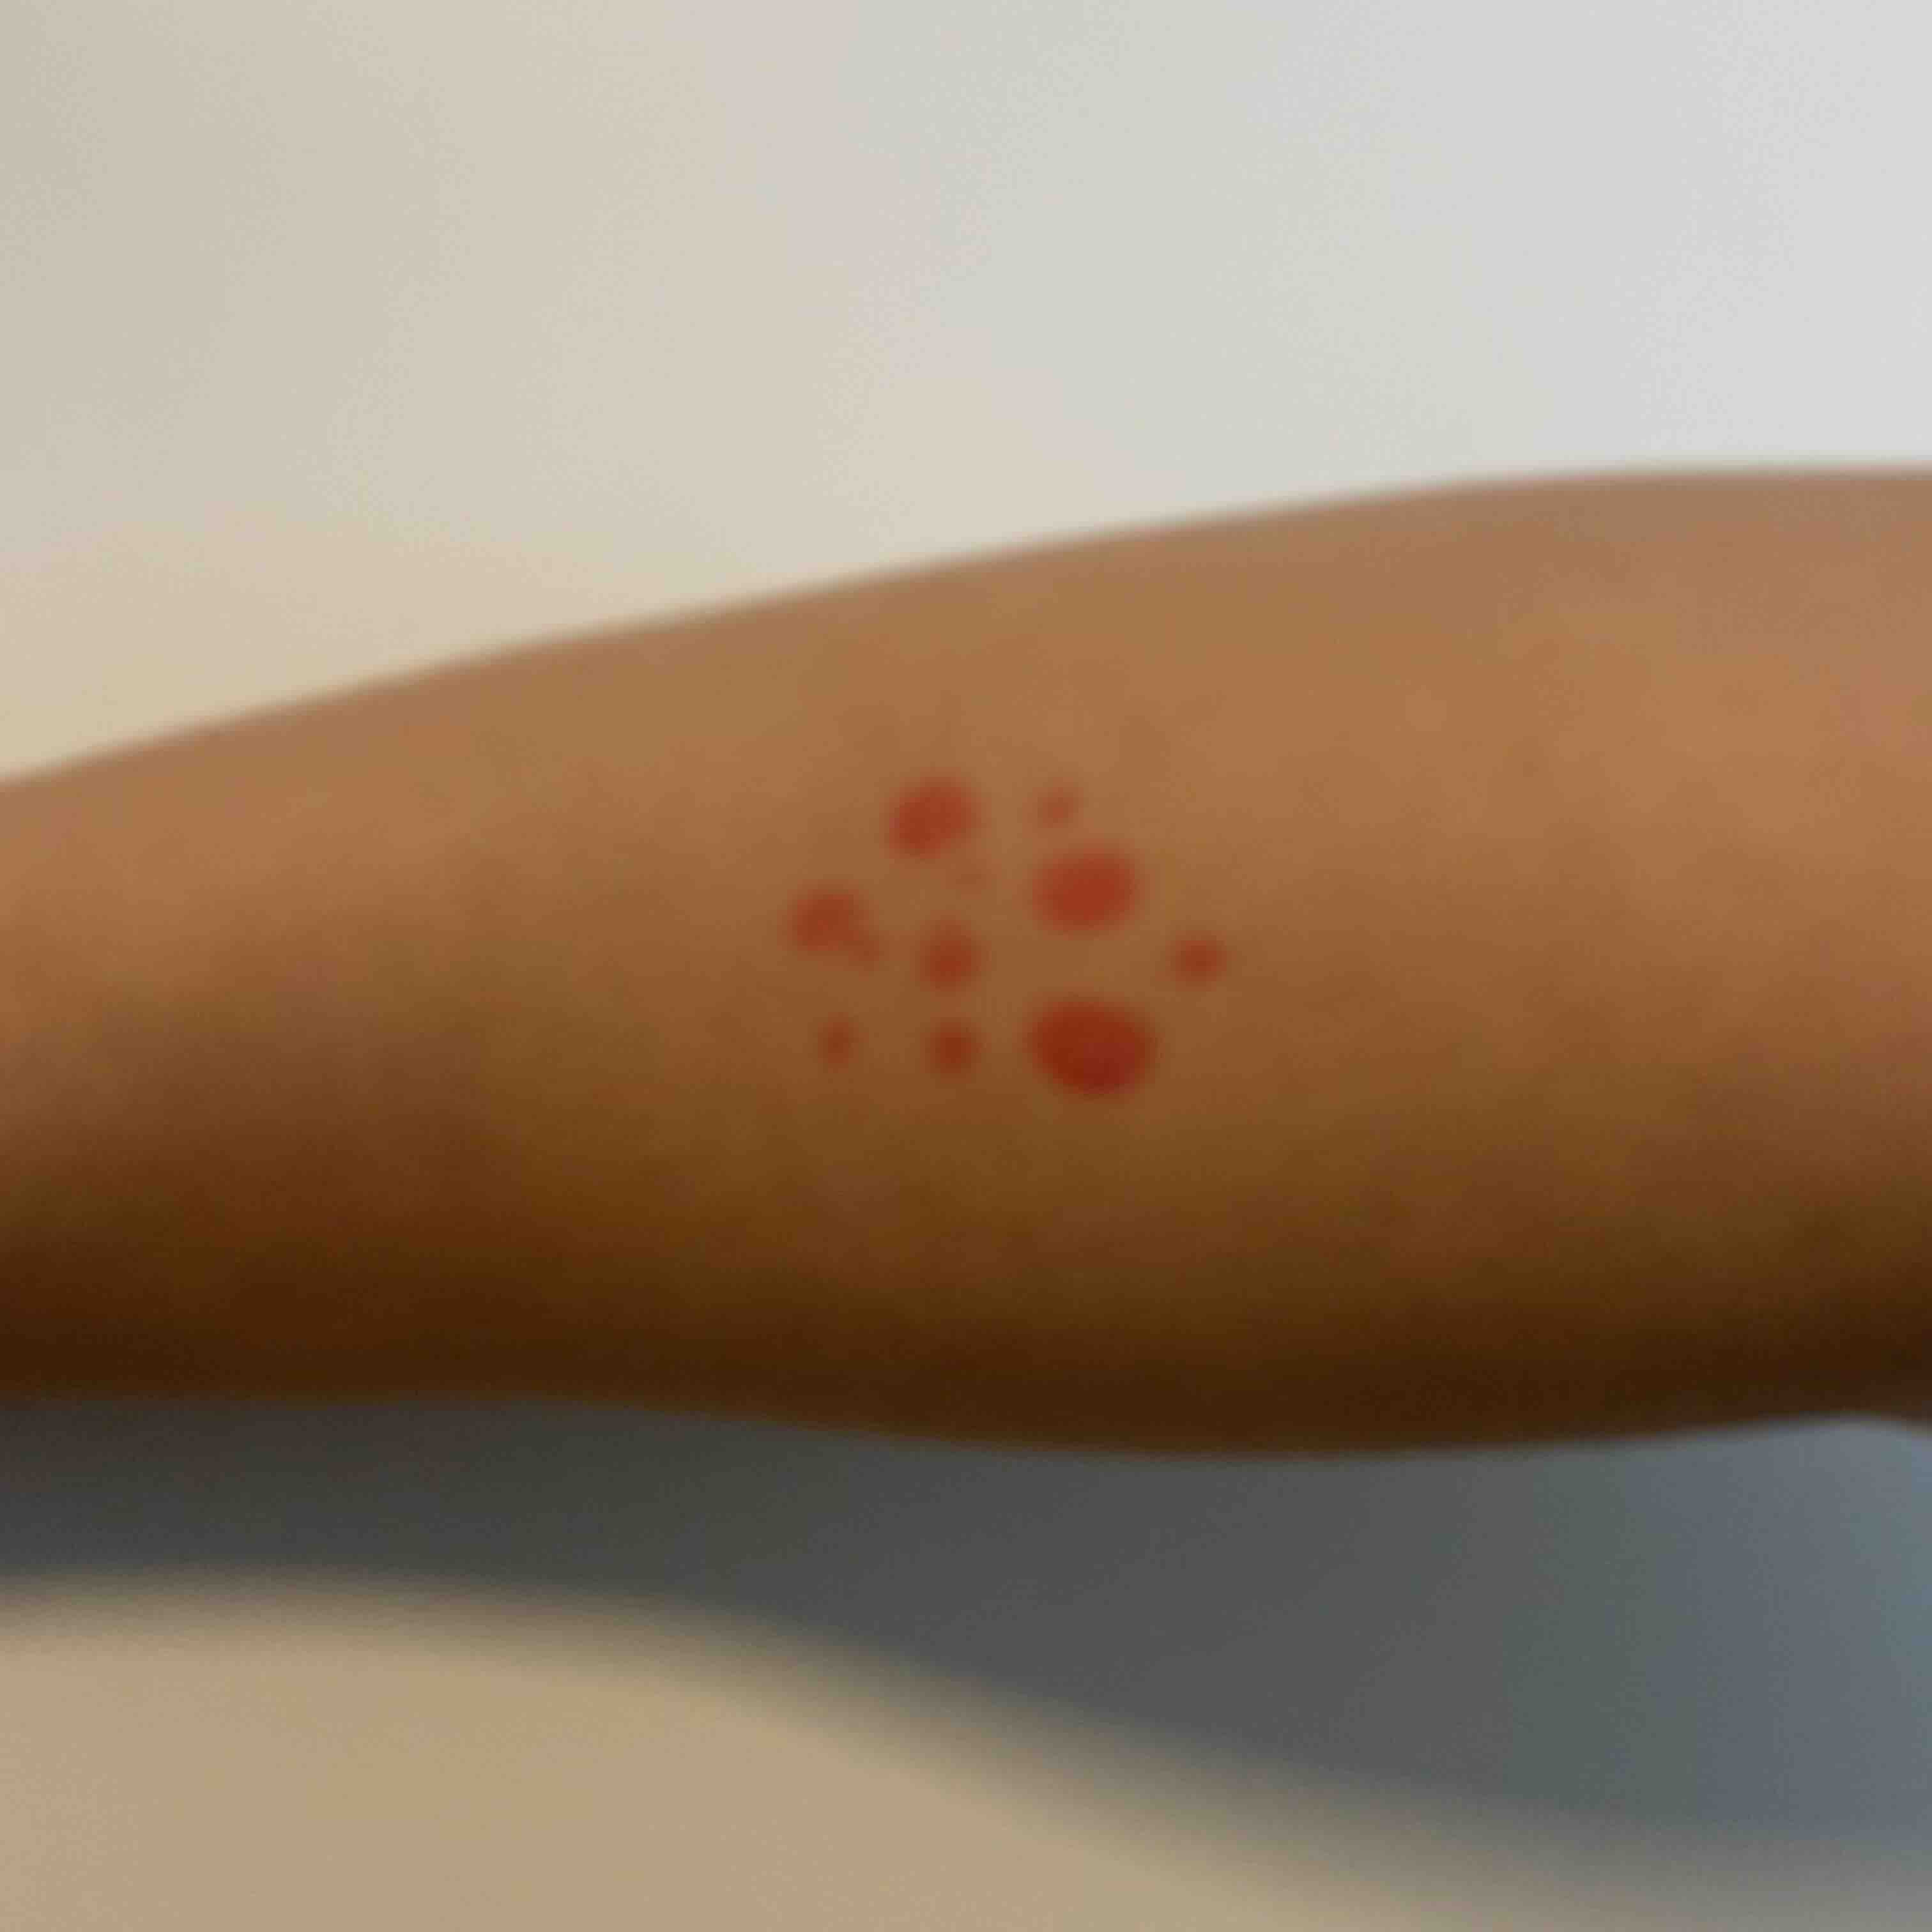
\includegraphics[width=\textwidth]{img/Focus.jpg}
        \caption{Focus}
        \label{fig:focus}
    \end{subfigure}
    \hfill
    \begin{subfigure}[b]{0.24\textwidth}
        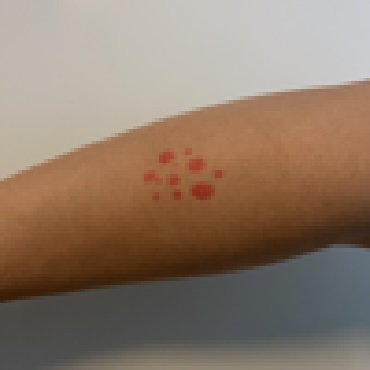
\includegraphics[width=\textwidth]{img/Resolution.jpg}
        \caption{Resolution}
        \label{fig:resol}
    \end{subfigure}
    \hfill
    \begin{subfigure}[b]{0.24\textwidth}
        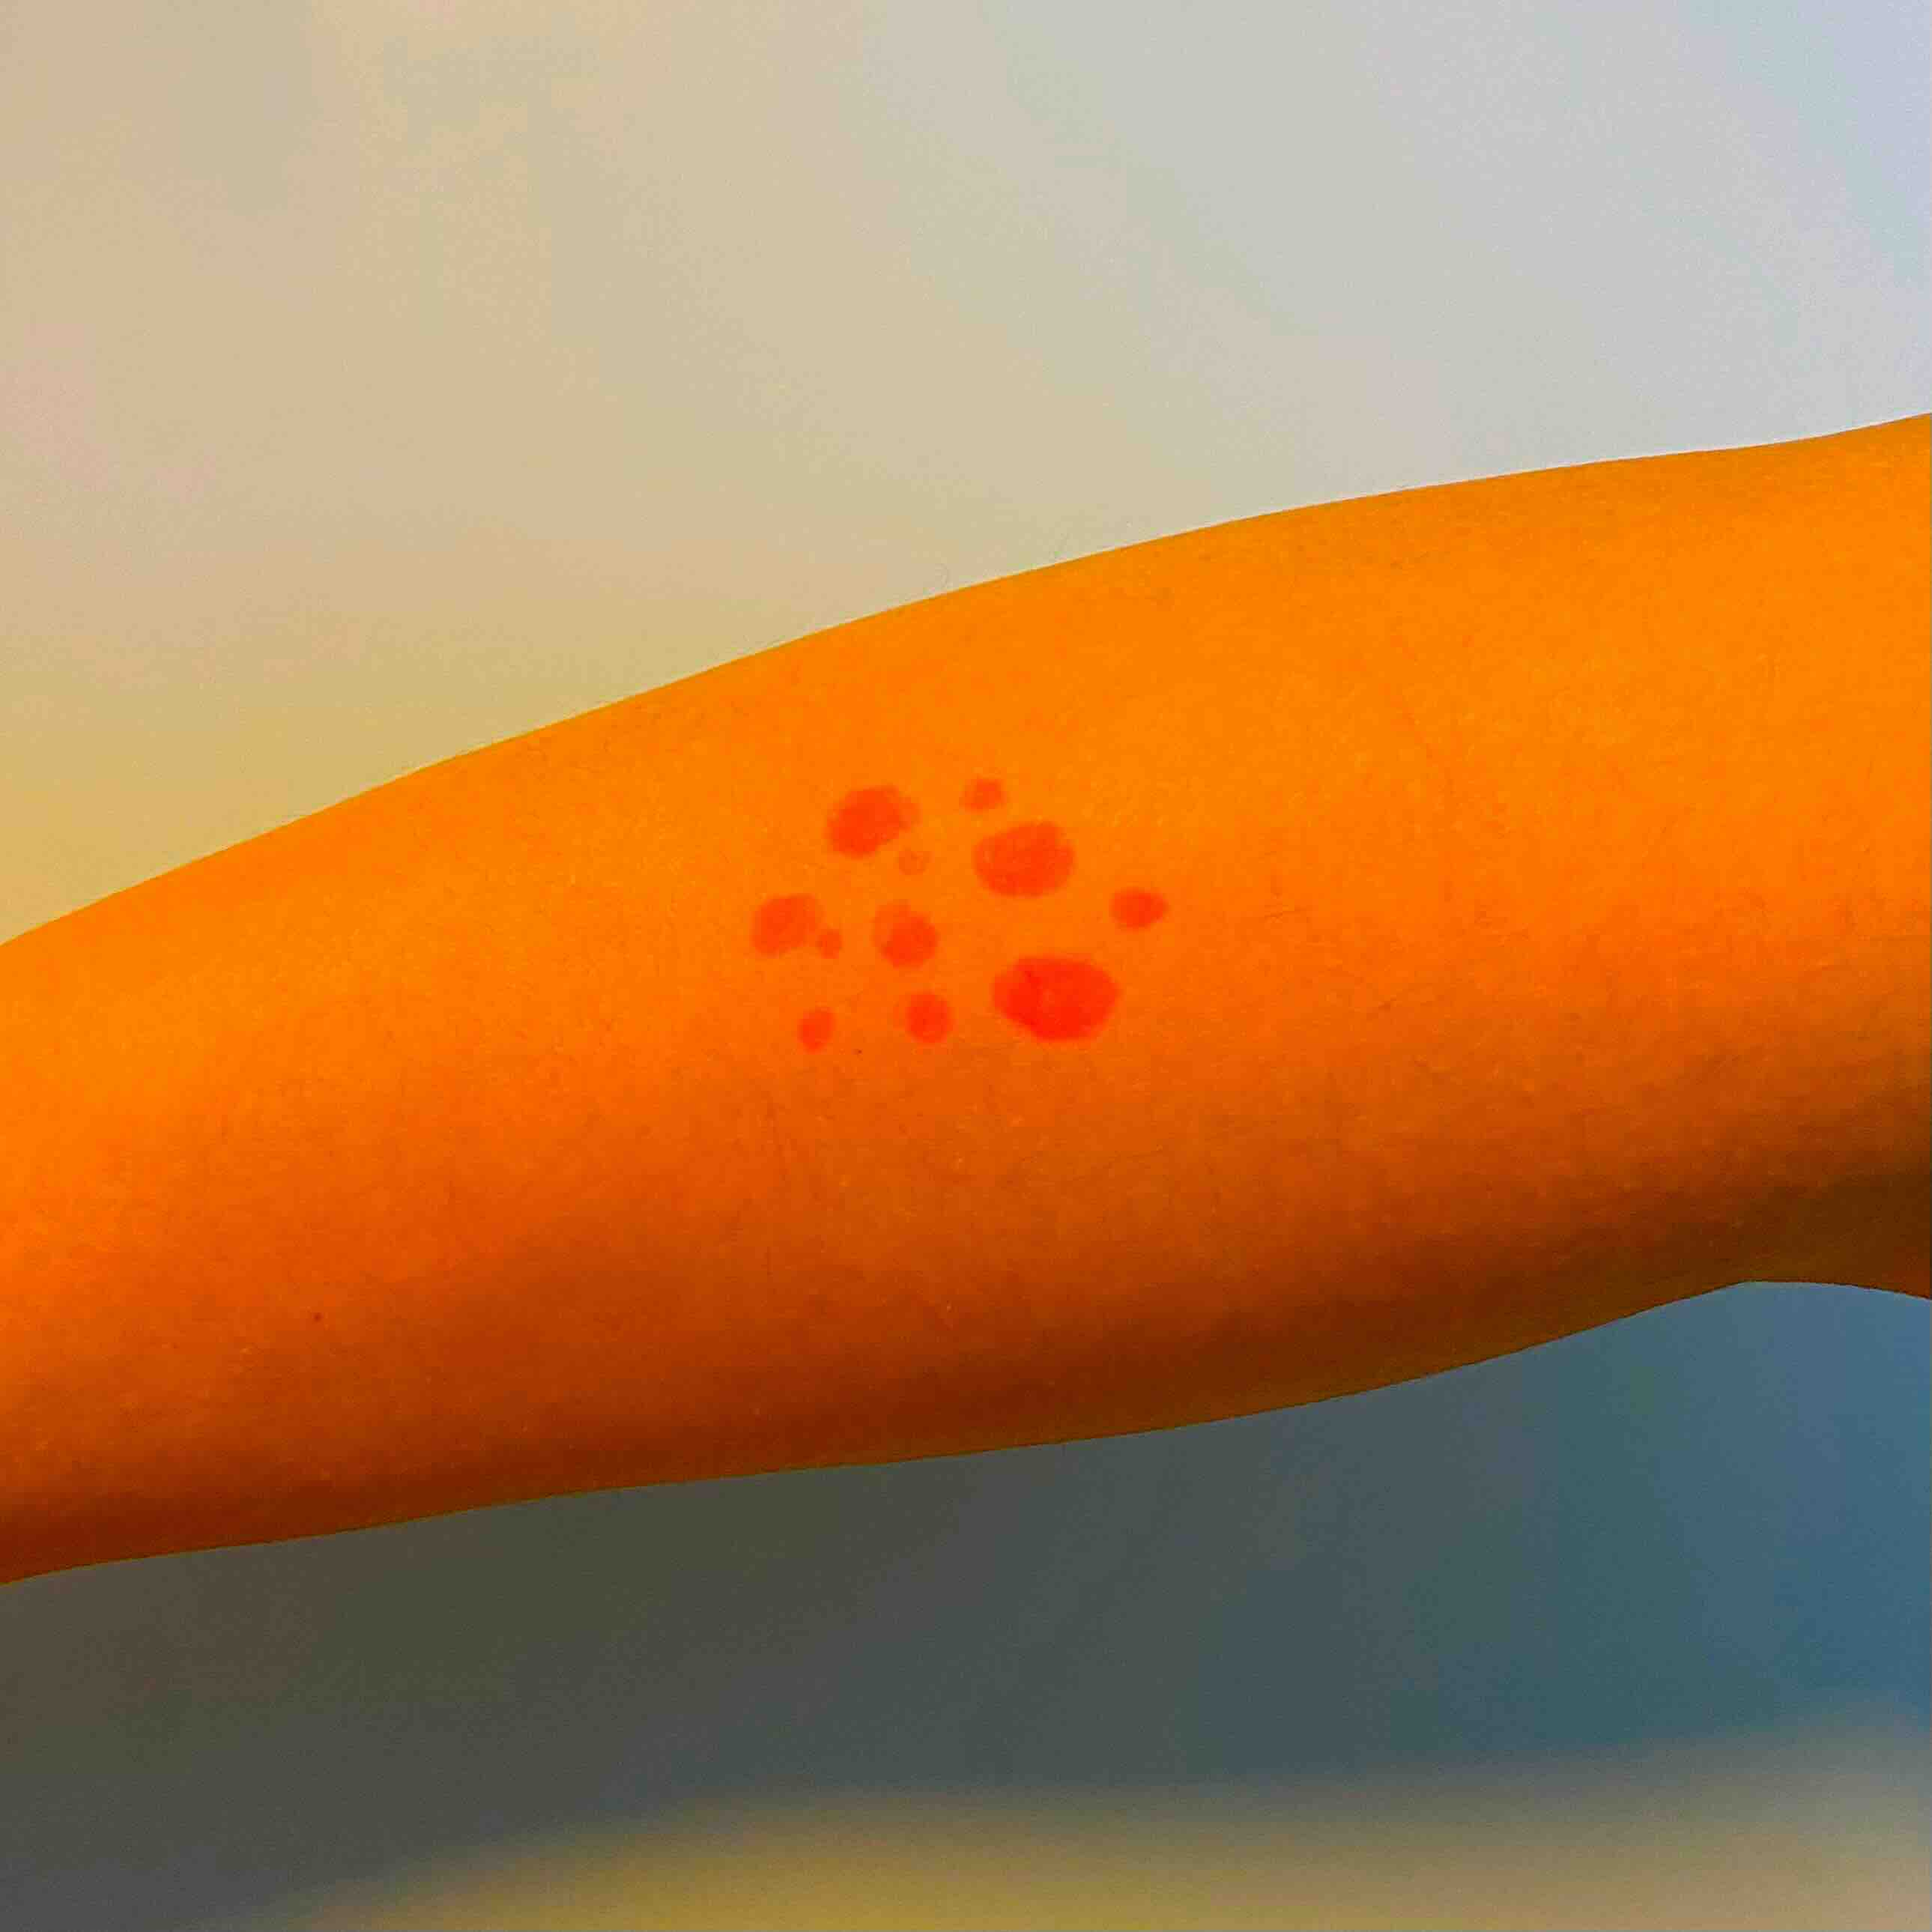
\includegraphics[width=\textwidth]{img/Color.jpg}
        \caption{Color Calibration}
        \label{fig:cc}
    \end{subfigure}
    \caption{Example images illustrating common distortions used in Teledermatology Image Quality Assessment. (Created by the Author)}
    \label{fig:quality_criteria}
\end{figure}
\begin{enumerate}
    \item \textbf{Lighting}:  Adequate illumination is critical. It should be even and diffuse, avoiding harsh shadows or overexposure that could obscure skin lesions or lead to misinterpretation of the skin's condition. \textbf{Remark} Position the light source evenly to avoid shadows and overexposure. Natural light or diffused artificial light can help illuminate the skin lesion uniformly and reduce glare.
    \item \textbf{Background}: A neutral and uncluttered background helps to focus attention on the dermatological issue without distraction, ensuring that the skin lesion is the most prominent feature in the image. \textbf{Remark} Use a plain, non-reflective background to minimize distractions and ensure the focus remains on the skin lesion. A neutral-colored backdrop, such as white or gray, is ideal for providing contrast with the lesion.
    \item \textbf{Field of View}: The image should be framed to include a clear view of the lesion as well as sufficient surrounding area to provide context, which can be crucial for accurate diagnosis. \textbf{Remark} Center the skin lesion or area of interest within the frame to ensure complete coverage and avoid cutting off important details. Maintain a consistent distance between the camera and the skin to prevent distortion.
    \item \textbf{Orientation}: Proper orientation of the image is vital. It should align with standard anatomical positions, allowing the dermatologist to easily interpret the image in relation to the patient's body. \textbf{Remark} Orient the camera perpendicular to the skin surface to capture images in the correct orientation. Align the camera with the skin lesion to maintain consistency and facilitate accurate comparison between images.
    \item \textbf{Focus \& Depth of Field}: Sharp focus on the lesion is a necessity, with a depth of field that keeps the entire area of interest in clear detail, as blurring can mask important characteristics of skin conditions. \textbf{Remark} Ensure the camera is in focus and adjust the aperture to achieve sufficient depth of field. Focus on the skin lesion to capture sharp, detailed images without blurriness or loss of clarity.
    \item \textbf{Resolution}: The image must be high resolution to reveal fine details of the skin. A higher pixel count can facilitate a more thorough examination and better clinical decision-making. \textbf{Remark} Use a camera with high-resolution capabilities to capture fine details and nuances of the skin lesion. Adjust the camera settings to the highest resolution possible to ensure clarity and precision in the image.
    \item \textbf{Color Calibration}:  Accurate color reproduction is necessary for the assessment of skin lesions. Any color distortion can lead to misdiagnosis, especially in conditions where hue is a diagnostic clue. \textbf{Remark} Calibrate the camera settings to accurately reproduce colors and skin tones. Avoid harsh lighting or color casts that may distort the color representation of the skin lesion. Use a color reference chart or white balance settings to ensure color accuracy.
\end{enumerate}
Each of these quality criteria contributes to the diagnostic accuracy in teledermatology by ensuring that the images convey the true nature of the skin condition. Just as in traditional dermatology, where the dermatologist's visual assessment is a key diagnostic tool, in teledermatology, the image serves as the eyes of the dermatologist. Therefore, optimizing these criteria is crucial to the successful application of teledermatology services.


\subsection{Teledermatology Datasets}
\label{sub:DatasetsTD}
The following datasets are valuable resources for teledermatology research and applications, especially notable for their accessibility and diversity. These datasets are not strictly confined to clinical settings or dermoscopic images and include patient-taken images, making them highly relevant for practical teledermatology purposes where clinical settings may vary:
\begin{itemize}
    \item \textbf{ACNE04}: This dataset focuses on acne severity and lesion counting, containing 1,457 images with detailed annotations for training and testing purposes \autocite{ACNE04}.
    \item \textbf{DDI}: Provides 656 high-quality images curated by dermatologists for detailed skin tone evaluation and diagnostic accuracy \autocite{DDI}.
    \item \textbf{Derm7pt}: Utilizes 1,011 lesion cases to train a neural network for classifying skin lesions and melanoma using the 7-point checklist \autocite{Derm7pt}.
    \item \textbf{Fitzpatrick17k}: Includes 16,577 images annotated for Fitzpatrick skin type across 114 different skin conditions \autocite{F17K}.
    \item \textbf{Monkeypox Dataset 2022}: Contains approximately 1,905 images focused on monkeypox, useful for developing diagnostic tools \autocite{Monkeypox}.
    \item \textbf{PAD-UFES-20}: Comprises 2,298 clinical images from smartphones, enriched with clinical metadata for comprehensive research \autocite{PAD-UFES-20}.
    \item \textbf{SCIN}: Emerged from a crowdsourcing initiative, this dataset contains 10,408 images capturing a broad spectrum of dermatological conditions \autocite{SCIN}.
\end{itemize}
\vspace{\baselineskip}
\noindent
These datasets collectively contribute to the advancement of teledermatology by providing varied, real-world data crucial for developing effective diagnostic tools and algorithms. \par 

\subsection{Approaches to Image Quality Assessment in Teledermatology}
\label{sub:ApproachesIQAinTeledermatology}
To understand the various approaches to Image Quality Assessment (IQA) within teledermatology, it is instructive to review related works that have contributed to the field. These studies not only offer insights into the methodologies employed for assessing image quality but also highlight the specific image distortions that are often targeted. Furthermore, by examining the architectures of the algorithms and the criteria used to classify image quality, we can discern the strengths and weaknesses of each approach. \par

\subsubsection{TrueImage: A Machine Learning Algorithm to Improve the Quality of Telehealth Photos}
\label{subsub:TrueImage}
The TrueImage algorithm prioritizes real-time, interactive feedback for patients taking dermatological images via their smartphones. Its three-stage process includes semantic segmentation to identify skin regions, feature generation focusing on blur, lighting, and zoom, and logistic regression classifiers that predict image quality and specific reasons for poor quality \autocite{TrueImage}. \par
\vspace{\baselineskip}
\noindent
The prototype exhibits promise, demonstrating the capability to reject approximately half of sub-par quality images while retaining around 80\% of good quality images. This suggests its potential utility in a clinical setting, where it could save time for both clinicians and patients by pre-screening image quality and offering specific feedback to improve poor submissions \autocite{TrueImage}.
\par
\vspace{\baselineskip}
\noindent
Yet, TrueImage’s current limitation lies in its modest dataset and the training data's lack of diversity regarding skin types, which could lead to biased quality assessments. Furthermore, while the algorithm excels at detecting blurriness, it is less effective at assessing lighting conditions and zoom, which are critical factors in teledermatology \autocite{TrueImage}.\par

\subsubsection{ImageQX: Explainable Image Quality Assessments in Teledermatological Photography}
\label{subsub:ImageQX}
ImageQX offers an automated, deployable method for IQA in teledermatology, addressing common image distortions: such as poor framing, bad lighting, blur, low resolution, and distance issues. With an architecture that employs the EfficientNet-B0 as a lightweight feature extractor. The network then employs linear layers, batch normalization, and dropout layers to predict poor image quality reasons, integrating them to forecast overall image quality \autocite{ImageQX}.
\par
\vspace{\baselineskip}
\noindent
The approach is data-driven, validated on a substantial dataset annotated by dermatologists, which underscores its potential for real-world applicability. With a macro F1-score of 0.73 for image quality assessment, ImageQX demonstrates expertise comparable to dermatologists and a capability for explainability via attention maps that can guide patients to retake pictures more effectively \autocite{ImageQX}.
\par
\vspace{\baselineskip}
\noindent
However, while ImageQX achieves high specificity, suggesting minimal disruption to patient experience by incorrectly rejecting high-quality images, its predictive performance for certain poor quality explanations like 'bad framing' remains low, with an F1-score of 0.37 \autocite{ImageQX}. This indicates room for improvement in addressing certain types of distortions, though the network’s size (15MB) makes it an attractive option for mobile deployment.
\par
\vspace{\baselineskip}
\vspace{\baselineskip}
\noindent
ImageQX stands out with its deep learning approach that uses a convolutional neural network (CNN) trained on a dataset of images labeled for quality by board-certified dermatologists. The network architecture is based on the lightweight EfficientNet-B0, which facilitates deployment on mobile devices. This model's training utilized a large dataset of 36,509 images, where the photographs were annotated for common quality issues, such as framing, lighting, blur, resolution, and distance from the subject.
\par
\vspace{\baselineskip}
\noindent
The strength of ImageQX lies in its explainability and its ability to provide reasons for poor image quality, aligning closely with the common distortions identified by dermatologists. It achieves a high macro F1-score, suggesting that its performance in image quality assessment is on par with expert human raters. However, some limitations include the difficulty of explaining certain quality issues like 'blurry' images, which had lower inter-rater agreement scores. The model's reliance on dermatologist-annotated images also points to the importance of the quality and diversity of the training dataset for its generalizability and accuracy. \par
\vspace{\baselineskip}
\noindent
In conclusion, both ImageQX and TrueImage present pioneering steps towards automated IQA in teledermatology, each with strengths such as deployability and real-time feedback capabilities. Their current challenges include the need for more diverse training data, improved detection of certain distortions, and further validation in real-world settings. Addressing these challenges will be crucial for their successful integration into teledermatological practices, ultimately contributing to more efficient and effective remote dermatological care. \par

\subsection{Challenges and Opportunities in Teledermatology}
\label{sub:ChallengesOpportunitiesTeledermatology}
Teledermatology has fundamentally changed how dermatological care is accessed, particularly in remote or underserved areas. However, the field faces several challenges that intersect with the focus of this thesis on image quality assessment.\par
\vspace{\baselineskip}
\noindent
One major challenge is the variability in image quality, which stems from patients using a wide range of devices in uncontrolled environments to capture images. This variability can severely impact the consistency and reliability of diagnoses made remotely. Additionally, technological barriers such as disparities in access to high-quality digital devices and varying levels of digital literacy among patients can further affect the quality of submitted images. Moreover, ensuring the privacy and security of sensitive dermatological images transmitted over the internet remains a critical concern that needs continuous attention to safeguard patient data.\par
\vspace{\baselineskip}
\noindent
On the opportunity front, recent advancements in image processing and machine learning technologies present significant potential to automatically enhance image quality and correct common distortions. This can greatly aid in improving diagnostic accuracy and efficiency. There is also a considerable opportunity to develop and implement standardized guidelines for image capture in teledermatology. Such standardization can help minimize quality variability and streamline the diagnostic process. Furthermore, the integration of artificial intelligence to provide real-time feedback to patients on improving image quality can enhance the effectiveness of teledermatology services by ensuring that only high-quality images are evaluated by dermatologists.\par
\vspace{\baselineskip}
\noindent
By tackling these challenges and leveraging the emerging opportunities, teledermatology can continue to evolve and play a crucial role in modern healthcare, enhancing access and efficiency in dermatological care across diverse populations.\par